%%=======================================================================
%% HOINet —— 《计算机学报》中文稿
%% 本文件由英文稿 mtap_en/paper.tex 逐节对应翻译而来，章节、图表、
%% 公式编号与英文稿一一对应，便于中英两版对照修改。
%%=======================================================================

\documentclass[10.5pt,compsoc,UTF8]{CjC}
% 本地 CjC.cls 已把内置字号命令统一改名为 \CjCzihao：CTEX 的 \zihao 用
% "-4" 表示小四，而本模板用 "4-" 表示小四，两套语法不兼容，不能共存。
% 这里的做法是让 CTEX 正常定义 \zihao，随后再把 \zihao 指回模板的
% \CjCzihao，从而恢复《计算机学报》模板的字号语义。
\usepackage{CTEX}
\let\zihao\CjCzihao
\usepackage{graphicx}
\usepackage{tabularx}
\usepackage{footmisc}
\usepackage{subfigure}
\usepackage{url}
\usepackage{multirow}
\usepackage{multicol}
\usepackage[noadjust]{cite}
\usepackage{amsmath,amsthm}
\usepackage{amssymb,amsfonts}
\usepackage{booktabs}
\usepackage{color}
\usepackage{float}
\usepackage{fancyhdr}
\usepackage{xcolor,stfloats}
\usepackage{comment}
\usepackage{cuted}
\usepackage{epstopdf}
\usepackage{gbt7714}
\usepackage{arydshln}
\graphicspath{{figures/}}
% 题注名与题注字体都放在这里改，不能写在导言区顶层：
% 本文件里 \figurename 被后注册的 AtBeginDocument 钩子改成了 "figure~"，
% 顶层 \renewcommand 会先执行、随后被覆盖掉（\tablename 没被动，一直是"表"）。
% 本钩子在类文件和 CTEX 之后注册，最后执行，改得动。
\AtBeginDocument{\renewcommand{\figurename}{图}%
  \renewcommand{\tablename}{表}%
  \captionnamefont{\small\heiti}%
  \captiontitlefont{\small\heiti}}

%=======设置奇偶页页眉=======%
\headevenname{\mbox{\quad} \hfill  \mbox{\zihao{5-}{计\quad \quad 算\quad \quad 机\quad \quad 学\quad \quad 报} \hspace {50mm} \mbox{2026 年}}}%
\headoddname{? 期 \hfill 李振等：符号的轴不是规模}
%=======设置奇偶页页眉=======%

\renewcommand{\thefootnote}{\fnsymbol{footnote}}
\setcounter{footnote}{0}
\renewcommand\footnotelayout{\zihao{5-}}
\newtheoremstyle{mystyle}{0pt}{0pt}{\normalfont}{1em}{\bf}{}{1em}{}
\theoremstyle{mystyle}
\renewcommand\figurename{figure~}
\renewcommand{\thesubfigure}{(\alph{subfigure})}
\newcommand{\upcite}[1]{\textsuperscript{\cite{#1}}}
\renewcommand{\labelenumi}{(\arabic{enumi})}
\newcommand{\tabincell}[2]{\begin{tabular}{@{}#1@{}}#2\end{tabular}}
\renewcommand{\bibsection}{}
\makeatletter
\renewcommand{\@biblabel}[1]{[#1]\hfill}
\makeatother
\setlength\parindent{2em}

\pagestyle{CjCheadings}
\setmainfont{Times New Roman}

% 待补充内容的醒目标记：红字加粗。定稿前应全部替换为真实信息。
\newcommand{\dk}[1]{{\color{red}\textbf{【待补：#1】}}}

%===========================================================%
% 放宽浮动体参数：本文图表多为跨两栏的宽幅图，默认阈值下会被一路推到文末。
\setcounter{topnumber}{3}
\setcounter{dbltopnumber}{3}
\renewcommand{\topfraction}{0.92}
\renewcommand{\dbltopfraction}{0.92}
\renewcommand{\textfraction}{0.06}
\renewcommand{\floatpagefraction}{0.72}
\renewcommand{\dblfloatpagefraction}{0.72}

% gbt7714 会加载 natbib，默认按 author-year 解释 \bibitem；本文是手写的
% 数字制 thebibliography，必须显式要求数字模式，否则 natbib 报
% "Bibliography not compatible with author-year citations"。
\setcitestyle{numbers}
% 模板把 \bibsection 清空了（\renewcommand{\bibsection}{}），文献表因此
% 没有标题。恢复成标准节标题，由 LaTeX 负责分页与间距 —— 手工加一行
% \noindent 会被排到页眉位置、与页码叠印。
\renewcommand{\bibsection}{\section*{参考文献}}
% ---- 正文用到的自定义宏（取自 slim/04_论文/latex/preamble.tex）----
\newcommand{\Dstar}{\mathcal{D}^{*}}
\newcommand{\PKD}{\mathrm{PKD}}
\newcommand{\dlt}{\Delta}
\newcommand{\pp}{\,\mathrm{pp}}
\DeclareRobustCommand{\code}[1]{\texttt{\spaceskip=0pt plus 0.4em\relax#1}}
\DeclareRobustCommand{\codesplit}[1]{\texttt{\spaceskip=0pt plus 0.4em\relax#1}}
\newcommand{\pthbreak}[1][0pt]{\hspace{0pt}\allowbreak\hspace{0pt}}

\begin{document}

%=======设置首页页眉=======%
\thispagestyle{empty}%
\begin{table*}[!t]
\vspace {-13mm}
\onecolumn
\noindent\begin{tabular}{p{168mm}}
\zihao{5-}
第??卷\quad 第?期 \hfill 计\quad 算\quad 机\quad 学\quad 报\hfill Vol. ??  No. ?\\
\zihao{5-}
20??年?月 \hfill CHINESE JOURNAL OF COMPUTERS \hfill ???. 20??\\
\hline\\[-5.5mm]
\hline\end{tabular}\end{table*}
%=======设置首页页眉=======%

%中文标题、作者与注脚
{
\centering
\vspace {11mm}
{\zihao{2} \heiti 符号的轴不是规模}

\vskip 3mm

{\zihao{4} \heiti ——多模态 RAG 中评测协议决定规模效应的符号}

\vskip 5mm

{\zihao{3}\fangsong 陈\quad 琳$^{1)}$ \quad 李\quad 振$^{1),\ast}$ \quad 王\quad 彬$^{1)}$ \quad 刘\quad 杰$^{2)}$}
\footnote{\noindent \zihao{6}\songti 收稿日期：\dk{年-月-日}；最终修改稿收到日期：\dk{年-月-日}. 本课题得到国家自然科学基金(62276155, 62572274)、山东省重点研发计划(2025CXPT091, 2025TSGCCZZB0792)与山东省人工智能教育研究课题(SDDJ202501088)资助. \textsf{陈琳}，\dk{性别}，\dk{出生年}年生，\dk{学位}，\dk{职称}，\dk{是否CCF会员及会员号}，主要研究领域为\dk{研究方向}、\dk{研究方向}.E-mail: chenlin@sdu.edu.cn. \textsf{李振(通信作者)}，\dk{性别}，\dk{出生年}年生，\dk{学位}，\dk{职称}，\dk{是否CCF会员及会员号}，主要研究领域为\dk{研究方向}、\dk{研究方向}.E-mail: jens@sdu.edu.cn. \textsf{王彬}，\dk{性别}，\dk{出生年}年生，\dk{学位}，\dk{职称}，\dk{是否CCF会员及会员号}，主要研究领域为\dk{研究方向}、\dk{研究方向}.E-mail: wangbin@sdu.edu.cn. \textsf{刘杰}，\dk{性别}，\dk{出生年}年生，\dk{学位}，\dk{职称}，\dk{是否CCF会员及会员号}，主要研究领域为\dk{研究方向}、\dk{研究方向}.E-mail: liuj1687@chinaunicom.cn.}

\vspace {1mm}

\zihao{6}{$^{1)}$(山东大学 数智化支撑研究院, 济南 250100)}

\zihao{6}{$^{2)}$(联通(天津)产业互联网有限公司, 天津 300110)}

\zihao{6}{$^{\ast}$通信作者.}
}%中文标题、作者与注脚

\vskip 5mm

\zihao{5-}{
\setlength{\baselineskip}{16pt}\selectfont{
\noindent {\heiti 摘\quad 要\quad }
检索证据与模型参数知识冲突时，RAG 行为不再只由任务难度决定。本文固定冲突构造、判定口径、模型与样本，只改 system prompt 对参数知识的授权强度，由弱到强预注册七档立场。在 927 条反事实编辑的冲突样本上，锚定协议保证五个规模点都知道该事实（$|D^*|=649$）。结果表明规模效应的符号由评测协议决定而非规模：七个立场的 $\Delta$ 跨零，符号沿授权序由负到正，跨度 47.5 至 56.5 pp，在两个模型族上复现；翻转由中段立场 \code{ctx\_hedge} 决定，故非单调梯度，且只在自由生成格式下成立。方法学上另报告三处方向明确的测量偏差——显式驳回被误记为不可判定、分母塌陷被误读为效应最强、位置偏好伪装成内容判断，每一处都足以让同一批数据给出相反结论。\par}}

\vspace {5mm}

\zihao{5-}{\noindent
{\heiti 关键词 \quad }检索增强生成；参数知识；知识冲突；模型缩放；评测协议；多模态大模型；预注册
}\par\noindent
\zihao{5-}{\heiti 中图法分类号\quad } TP391

\vskip 5mm

\begin{center}
\zihao{3}{ \heiti The Axis of the Sign Is Not Scale: Evaluation Protocol Determines the Sign of the Scale Effect in Multimodal RAG}\\
\vspace {5mm}
\zihao{5}{ Lin Chen$^{1)}$ \quad Zhen Li$^{1),\ast}$ \quad Bin Wang$^{1)}$ \quad Jie Liu$^{2)}$}\\
\vspace {1mm}
\zihao{6}{{$^{1)}$(Digital Intelligence Support Research Institute, Shandong University, Jinan 250100, China)}}

\zihao{6}{{$^{2)}$(China Unicom (Tianjin) Industrial Internet Co., Ltd., Tianjin 300110, China)}}
\end{center}

\zihao{5}{
{\noindent\bf Abstract}\quad Retrieval-augmented generation (RAG) is
effective on knowledge-intensive tasks, yet when retrieved content
conflicts with a model's parametric knowledge its behaviour is no longer
governed by task difficulty alone. This paper measures a variable that is
usually taken for granted in multimodal RAG: the sign of the effect of
model scale on resistance to a corrupted retrieval context. We hold the
conflict construction, the adjudication criterion, the models and the
samples fixed, and vary exactly one variable---the strength of the
system prompt's authorisation of parametric knowledge---pre-registering
seven stances ordered from weak to strong, from ``use the context only''
to ``prefer your own knowledge''. On the same 927 controlled
counterfactually edited conflict samples, an anchoring protocol
guarantees that every model scale genuinely knows the fact at issue
($|D^{*}|=649$), and we measure the rate at which each scale follows
parametric knowledge under each stance.

The sign of the scale effect is determined by the evaluation protocol,
not by scale. The $\Delta$ of the seven stances crosses zero, with signs
running from negative to positive along the pre-registered authorisation
order, spanning 47.5 to 56.5 percentage points, and replicating
independently on two model families. The ordering is \textbf{not} a
monotone gradient: the sign flip is decided by the mid-ladder stance
\code{ctx\_hedge}, while the semantically weaker neutral stance that
follows it yields almost no effect. That same cell is also the least
trustworthy in magnitude, and removing it leaves the sign sequence
unchanged while the rank correlation of one family rises from 0.643 to
1.000. A pre-registered prediction test confirms the sign claim and
falsifies the magnitude claim. The structure holds only under free
generation: under the forced-choice templates of two published works all
four conditions fall within $-4$ pp. Methodologically we report three
directional measurement biases---explicit rejection misread as
undecidable, denominator collapse misread as the strongest effect, and
position preference masquerading as content---each of which would let the
same data support the opposite conclusion. The measurement is limited to
five scale points, two model families and a single dataset, and the
mechanistic account is behavioural.
}

\vskip 3mm

% 由 cjc_build.py 自动生成，请勿手工编辑。

\section{引言}\label{sec:1}

检索增强生成把模型记不住的事实交给外部证据。但一旦检索内容与参数知识冲突，系统行为就不再由任务难度决定：同一道题、同一个模型，答出的可能是检索内容，也可能是参数里记着的那一个，而选哪一个取决于提示词怎么写。这在部署中不是边角情况——检索证据本可能出错。多模态场景把问题推得更远：图像证据、检索文本、参数事实三者可能两两冲突。近年一批工作开始测量这种选择，确立了“模型会被冲突上下文带偏”的现象\cite{ref1,ref2,ref3}，也留下了一个问题：这种带偏随模型能力增强是变好还是变坏？

一个自然的猜测是变好。但该猜测的检验有一个不易察觉的前提：它要求“规模”是唯一变化的变量。实际评测中提示词也在变，有的说“仅根据上下文回答”，有的说“若上下文不可靠则以自有知识为准”。若模板对参数知识的授权程度本身就会改变行为，把两个规模的差异归因于规模，可能是在测量模板。

本文把这个问题做成可判决的实验：固定冲突构造、判定口径、模型与样本，只改一个变量——system prompt 对参数知识的授权强度，按语义由弱到强预注册为七档。在同一批 927 条受控反事实编辑的冲突样本上，测量每个规模、每个立场下模型跟随参数知识的比例；并用锚定协议保证所有被测规模都确实知道该事实，把 927 条收缩到 649 条，从而把“能力差距”从“大模型多知道几个事实”这一平凡解释中隔离出来。

结果是：规模效应的符号不由规模决定，而由立场决定。两个模型族上，弱授权立场下大规模模型更倾向跟随上下文（\code{ctx\_only} 分别为 $-27.3$ 与 $-8.4$ pp），强授权立场下更倾向坚持参数知识（\code{prior} 为 $+28.0$ 与 $+33.7$ pp）。两族的 $\Delta$ 都跨零，符号沿预注册授权序由负到正排列，在相邻规模对的分解中呈现早期饱和而非平滑增长。

符号的排列不是单调梯度——这是最容易被误读的一点。决定符号翻转的不是“授权越强、效应越正”：中段立场 \code{ctx\_hedge} 给出 Qwen3 族 $+29.2$ pp，而授权语义上更弱的纯中立立场只给出 $+1.5$ pp。符号落在哪个立场上，由该立场的输出形态与判定口径共同决定，这正是标题所说的“协议”而非“立场语义”。该格同时是量值最不可信的一格；把它整个拿掉，两族符号序列完全不变，跨度仅由 56.5 降至 55.3 pp。最不可信的那一格不是承重的。这个结论有一个必要的限定：它只在自由生成格式下成立，换成强制选择模板后四个条件的规模效应全部落在 $-4$ pp 以内（\ref{sec:4-4}）。

方法学层面，本文报告三个此前未被系统处理的测量问题，每一个都会让同一批数据给出方向相反的结论。其一，判据把显式驳回误记为不可判定，而这类答案恰是跟随参数知识最明确的一类；剔除量随规模上升，修正后某立场 \code{PKD} 从 0.359 升至 0.960。其二，分母塌陷被误读为效应最强：同一立场的配对可判样本数从 584 条塌到 1 条，本文因此规定 $n<50$ 的格不计入跨度与符号比较。其三，位置偏好可完全压倒内容：强制选择格式下互换选项后重跑，位置偏好达 $+0.961$，高准确率是位置偏好的产物而非内容判断。

本文的贡献有三。第一，给出“规模效应的符号是评测协议的函数”这一测量结论，并做成可判决的实验设计：七个预注册立场 × 五个规模点 × 两个模型族，$\Delta$ 跨零且符号有序，两族独立复现。第二，确立受控反事实编辑加锚定协议这一三元冲突测量构造，使跨规模比较有确定的语义。第三，系统报告并修正三个方向明确的测量偏差。边界也需如实说明：测量只在五个规模点、两个模型族、单一数据集上完成，机制解释是行为层的。发现负号与正号方向的工作各有其先，“效应符号可跨零”也已有人沿模型尺寸轴报告\cite{ref7}；本文不主张这两项的首发权，主张的是“跨零的轴是评测协议而非模型尺寸”这一正交性结论。

由于篇幅限制，其他材料及代码可在 github 查看 \url{https://github.com/data-echo-20/slim-eval-protocol}。

\section{相关工作}\label{sec:2}

\subsection{参数知识与上下文的冲突}
\label{sec:2-1}

模型在上下文与参数知识不一致时的选择，是知识冲突研究的出发点。ConflictBank\cite{ref1} 构造了 745 万条声明-证据对、55.3 万条问答对；Longpre 等\cite{ref2} 把冲突形式化为实体层面的“上下文对参数”冲突，并论证对记忆信息的过度依赖是幻觉成因之一；ClashEval\cite{ref4} 报告模型采纳错误检索内容的比例超过 60\%。机制层面，Yao 等\cite{ref18} 与 Pham 等\cite{ref20} 用知识电路与分层注意力归因表明，这一竞争发生在可定位的中间层。这些工作测量的都是模型“被带偏的频率”；本文测量的是符号方向与跨立场的有序性，并引入三元冲突结构——反事实编辑同时提供篡改的检索文本、图像证据与参数知识三路候选。

\subsection{规模作为自变量}
\label{sec:2-2}

规模与能力的非单调关系已有刻画：Kaplan 等\cite{ref5} 发现损失随规模呈幂律下降，McKenzie 等\cite{ref6} 报告 U 形与倒 U 形趋势。与本文最相关的是规模与指令服从的交互。De Marez 等\cite{ref7} 在 56 个开放权重模型上测量社会压力下的事实迎合，发现指令微调的优势随规模反号、在 7B 附近跨零。该文沿模型尺寸轴跨零而固定评测协议，本文沿协议轴跨零而固定模型族与样本；它的 13 类操纵全在社会压力框架内，因变量是固定二选一选项的对数概率差，结构上不存在弃权态，全文无 system prompt 授权强度的操纵、无剂量-反应、无长度控制。它已用同一套统计语言报告了 7B 处的跨零，故本文不主张首创“效应符号可跨零”这一现象本身，主张的是把跨零的轴换掉。它把跨零解释为阈值假象（抹去两通道均值差后交互方差份额下降约 79.9\%），本文的反制有三项：跨协议复用同一题集、做逐项符号检验而非仅比较聚合均值、用弃权口径作为第二条独立曲线。规模与微调还相互纠缠：Zhou 等\cite{ref21} 用指令数据训练模型在参数知识与上下文之间取舍，Gekhman 等\cite{ref29} 则报告微调注入的新知识与幻觉率正相关；本文换的是授权而非格式\cite{ref30}。

\subsection{评测协议对结论的影响}
\label{sec:2-3}

同一批模型输出在不同评测协议下可以被判为不同的行为。迎合与指令服从的测量对措辞敏感：Sharma 等\cite{ref8} 把事实迎合归因于人类偏好偏向迎合性回复，Turpin 等\cite{ref9} 表明选项重排等偏置可移动答案多达 36\%。检索侧，Asai 等\cite{ref24}、Wang 等\cite{ref22}、Huang 等\cite{ref23} 分别用自评检索、迭代式筛选与有条件的信任来消除冲突；本文不消除它，而是把它当作测量工具。检索增强下的推理失败还可归因于检索器与语言模型的分工\cite{ref25}；迎合另有训练侧的来源，用合成数据可以把它压下去而不损失通用能力\cite{ref41}，而它从事实层面扩展到社会层面后与奖励篡改相连\cite{ref42,ref43}。有两项工作与本文题目最接近。Pandere 等\cite{ref10} 对 base 与 instruct 模型做电路级归因，把指令微调刻画为把模型推向参数记忆，且指出其效应对连贯证据段落会消失，即一个 framing 因素。Bhowal 等\cite{ref15} 在医学视觉语言模型上区分两种“模型自有推理”的操作化，同一段文本在“占据模型自己的 token 位置”下采纳约 73.5\%、在“仅贴来源标签”下约 16.0\%；它把方向复现当作稳健性证据，而本文主张的是符号随协议强度跨零翻转。两文的共同差别在于：它们的协议轴都是二元的，而本文的授权强度是七档预注册的有序变量；且两者都没有做跨零检验。

\subsection{多模态条件下的对应问题}
\label{sec:2-4}

多模态条件把该问题推进到视觉证据。Liu 等\cite{ref11} 在 374 张图像、1122 条问答对上报告约 20\% 的查询上模型过度依赖参数知识而非矛盾的视觉证据；CC-VQA\cite{ref12} 是免训练的缓解方法。诊断类工作中，Tang 等\cite{ref13} 把多模态长链推理的冲突分为输入层与过程层两类并报告方向不对称；Lee 等\cite{ref14} 发现同一语义以图像给出比以文本给出时更易被矛盾上下文带偏；Li 等\cite{ref34} 用轮询式判别查询把“看错”与“记错”分开测量。PENDULUM\cite{ref3} 把迎合测量扩展到视觉语言模型，其自变量是提问者提示的影响方向，而本文的自变量是对参数知识的授权强度。Aranya 等\cite{ref16} 把“接地”与“迎合”对立起来并报告负相关，但该工作把所有模型固定在同一量级且因变量全为非负量，故结构上无法跨零。

\section{数据与测量协议}\label{sec:data}

\subsection{数据集与筛选}
\label{sec:4-1}

\subsubsection{从 E-VQA 到两代锚定集}
\label{sec:4-1-1}

本文的评测集建立在 E-VQA 之上。该数据集的问题全部以“this plant”“this animal”
“this insect”这类指代性短语指代实体，实体身份只能由图像确定。这一设计在原始任务中
是优点，对本文要测的量却是障碍：把指代词原样喂给模型，它答出的是该类问题的语言先验，
而不是关于这个物种的知识。

症状在第一轮筛选中就暴露了。用原始问法筛出的 6 条所谓“强锚定”样本，全部落在同一个模板上，
\codesplit{I\allowbreak{}n\allowbreak{} w\allowbreak{}h\allowbreak{}i\allowbreak{}c\allowbreak{}h\allowbreak{} s\allowbreak{}e\allowbreak{}a\allowbreak{}s\allowbreak{}o\allowbreak{}n\allowbreak{} d\allowbreak{}o\allowbreak{}e\allowbreak{}s\allowbreak{} t\allowbreak{}h\allowbreak{}i\allowbreak{}s\allowbreak{} p\allowbreak{}l\allowbreak{}a\allowbreak{}n\allowbreak{}t\allowbreak{} g\allowbreak{}i\allowbreak{}v\allowbreak{}e\allowbreak{} f\allowbreak{}l\allowbreak{}o\allowbreak{}w\allowbreak{}e\allowbreak{}r\allowbreak{}s\allowbreak{}?\allowbreak{}} 一律答 \code{Spring}，而对应的物种是 6 个不同的种。
模型答对的是“什么时候开花”这个问题的常识分布，与它是否认得该物种无关。

对策是把指代词替换为物种名，再重新筛选。这一改动使命中率下降，但换来的是
“模型持有该事实”而非“模型熟悉该句式”的可靠测量。近期多模态知识冲突基准
同样把实体放在问题的中心\cite{ref31}，冲突的落点是模型对该实体的参数记忆与上下文
陈述之间的不一致。此后分两代扩展。两代锚定集的规模与筛选口径见表 S11（见在线材料）。

两代样本基本不重叠：927 条中仅 147 条属于 236 条。第一代用于把反事实编辑管线调通，
第二代才是本文的实验对象。区分二者是必要的，因为第一代是单模型筛选，
存在系统性的筛选偏倚——被 3B 知道的事实天然偏向高频、模板化的物种属性，
这类事实恰好也是大模型无需检索就能答对的。用这样的集合去比较规模，差异会被筛选口径吸走。

\subsubsection{第二代集合的构造}
\label{sec:4-1-2}

第二代集合的构造分三步。先从 E-VQA 候选池中取出带证据句的条目，用实体名问法重新提问，
再让 Qwen2.5-VL 的 3B 与 7B 各做一次无上下文回答，最后取两者都答出参数真值的样本。

第二步用两个规模而非一个，是因为本文的因变量是跨规模的行为差异。
若只用一个模型筛选，被选中的样本对该模型而言必然“已知”，
而另一个规模是否同样知道却未经检验。两个规模都确认知道，才能保证后续观察到的差异
不是“大模型多知道几个事实”这一平凡效应。

筛选后逐条做反事实编辑，共 1146 条进入有效池，其中 927 条的编辑结果通过质检，构成主实验集。
另 219 条因改写失败被剔除：编辑后语义自相矛盾、数字格式畸形、或编辑未能真正改变取值。
被剔除的样本 \codesplit{c\allowbreak{}o\allowbreak{}n\allowbreak{}t\allowbreak{}e\allowbreak{}x\allowbreak{}t\allowbreak{}\_c\allowbreak{}o\allowbreak{}n\allowbreak{}f\allowbreak{}l\allowbreak{}i\allowbreak{}c\allowbreak{}t\allowbreak{}} 字段为空，评测时喂进去的是与参数知识一致的上下文，
永远不可能表现出冲突行为——把它们留在分母里等于往 \code{PKD} 里掺零。

\subsubsection{反事实编辑管线}
\label{sec:4-1-3}

编辑的载体是证据句中的单个槽位，编辑后上下文与参数真值冲突，其余部分保持逐字不变。
单槽位替换是必要的：它让冲突位置可精确定位，从而使“模型是否察觉到冲突”
与“模型在哪个语义维度上让步”两件事可以分开考察。整段改写做不到这一点。
冲突注入与既有知识冲突基准同源\cite{ref17,ref19}，区别只在粒度：基线工作通常注入
整段冲突证据，本文只动一个槽位。

管线处理了四类事故。四类事故的处置明细见表 S1（见在线材料）。

最终质检结果为畸形数字 0、重复标点 0、编辑未生效 0。

\subsubsection{图像映射}
\label{sec:4-1-4}

236 条锚定样本全部配上 iNaturalist 2021 图像，映射链为三段：

\begin{quote}\ttfamily\small
\noindent wikipedia\_title --(学名一致)--> val.json.categories.name\\
\noindent -> categories.image\_dir\_name -> images.file\_name
\end{quote}

第一段的学名一致率实测 100\%。两处易错点记录如下。其一，\codesplit{d\allowbreak{}a\allowbreak{}t\allowbreak{}a\allowbreak{}s\allowbreak{}e\allowbreak{}t\allowbreak{}\_c\allowbreak{}a\allowbreak{}t\allowbreak{}e\allowbreak{}g\allowbreak{}o\allowbreak{}r\allowbreak{}y\allowbreak{}\_i\allowbreak{}d\allowbreak{}}
必须零填充为 5 位，否则目录名匹配失败。其二，\codesplit{d\allowbreak{}a\allowbreak{}t\allowbreak{}a\allowbreak{}s\allowbreak{}e\allowbreak{}t\allowbreak{}\_i\allowbreak{}m\allowbreak{}a\allowbreak{}g\allowbreak{}e\allowbreak{}\_i\allowbreak{}d\allowbreak{}s\allowbreak{}} 存的是 iNat
原始照片编号，不在竞赛发布的 10 万张之内，无法据此定位文件，必须走 \code{image\_dir\_name}
与 \code{file\_name} 两个字段。

\subsubsection{槽位构成}
\label{sec:4-1-5}

927 条主实验集的粗粒度槽位分布为 place 512 条、other 335 条、quantity 33 条、
diet 28 条、time 19 条。place 一类占 55.2\%，本文结论主要由地理类事实承载。
细粒度上，\code{edit\_slot} 的前三类为 place 507、city 281、quantity 44，
即地理槽位内部还进一步区分了国别与城市两级。

需要提醒读法：quantity 槽位在 927 集中仅 33 条，而在第一代 236 集中有 66 条，
占比从 28.0\% 降到 3.6\%。两代集合的槽位构成差异较大，故本文不做逐槽位的规模效应结论，
只在与 \ref{sec:4-7} 的分域检验并列时报告，且注明各组样本量。

规模比较不在 927 条上进行，而在其子集 $D^*$ 上，收缩幅度与理由见 \ref{sec:4-2-5}。

\begin{figure*}[t]
  \centering
  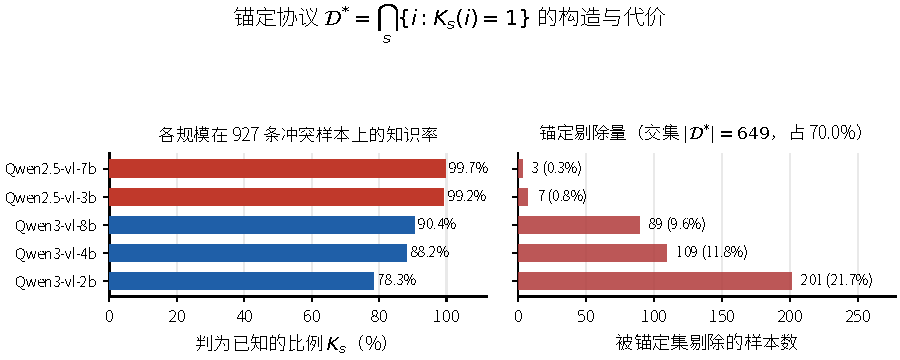
\includegraphics[width=\textwidth]{figures/fig04_anchoring.pdf}
  \caption{锚定协议 $\Dstar=\bigcap_s\{i:K_s(i)=1\}$ 的构造与代价。}
  \label{fig:anchoring}
\end{figure*}

如图~\ref{fig:anchoring} 所示，左图为各规模在共同覆盖冲突样本上判为已知的比例 $K_s$，右图为锚定剔除量。锚定集只保留所有规模点都判为已知的样本，代价是分母收缩，收益是消除“知识量随规模变化”这一背景条件。


\subsection{测量协议与实现细节}
\label{sec:4-3}

本章的全部结论都建立在一种测量上：给模型一段与它自身知识冲突的上下文，
看它跟随谁。这类测量对实现细节异常敏感，本文在预实验中发现三处选择会让
同一批样本量出完全不同的结果。把它们写在结果之前，是因为后面的每一个数字
都依赖它们；也是因为这三处错误在已发表工作中普遍存在，读者若不复现我们的
协议选择，就无法得到可比的数字。

\subsubsection{三条测量口径}
\label{sec:4-3-1}

\paragraph{口径一：无上下文臂必须配中性 system prompt}
\label{sec:xd513ea1621}

测“模型自己知道多少”时不能给上下文，但 system prompt 仍会悄悄影响测量。
若沿用有上下文臂的 system prompt（其中写着使用所给上下文），模型在本该
依赖自身知识的条件下收到的是“别太依赖自己”的暗示。实测在 236 条样本上，
用有上下文版的 system prompt 测得的参数知识率为 0.496，换成中性
system prompt 后为 0.9746。差异接近 48 个百分点，足以让“模型是否知道”
这一最基础的判断反向。

本文因此为无上下文臂单独使用中性提示：`You are a knowledge assistant.
Answer with a short phrase.`。有上下文臂的七种立场各有自己的措辞，见 \ref{sec:4-3-2}。

\paragraph{口径二：知识率只在纯文本臂上判读}
\label{sec:x17b8e010ee}

带图臂测的是“图像介入之后参数知识还剩多少”，本身不是知识持有量的无偏估计；
用它筛样本会把视觉干扰混进选择。本文的锚定集 $D^*$ 因此完全由纯文本臂构造，
视觉臂只用于 \ref{sec:4-6} 的对照。

\paragraph{口径三：冲突条件的有效分母必须排除改写失败样本}
\label{sec:x357e5e1775}

口径三同 \ref{sec:4-1-2}：改写失败的样本上下文与参数知识一致，永远无法表现出冲突
行为，算进分母等于往 \code{PKD} 里掺零，故冲突条件的有效分母去掉 219 条后为 927 条。

\subsubsection{七种指令立场}
\label{sec:4-3-2}

七种立场只改 system 与 user 模板的措辞，样本、上下文、图像、解码参数完全不动。
表~\ref{tab:stance-ladder} 给出逐字定义与授权强度。授权强度是对参数知识的授权程度，由弱到强预注册排序，
排序在见到数据之前写定。

\begin{table*}[t]
  \caption{七种指令立场的逐字定义与授权强度}
  \label{tab:stance-ladder}
  \centering
  \footnotesize
  \setlength{\tabcolsep}{3pt}
  \setlength{\arrayrulewidth}{0.4pt}
  \begin{tabularx}{\linewidth}{>{\raggedright\hsize=0.4497\hsize\arraybackslash}X>{\raggedright\hsize=1.3821\hsize\arraybackslash}X>{\raggedright\hsize=1.1682\hsize\arraybackslash}X}
    \toprule
    立场 & system prompt & user 模板 \\
    \midrule
    \code{ctx\_only} & \code{...that \pthbreak{}relies \pthbreak{}solely \pthbreak{}on \pthbreak{}the \pthbreak{}provided \pthbreak{}context.\pthbreak{}} & \code{Answer \pthbreak{}briefly \pthbreak{}using \pthbreak{}only \pthbreak{}the \pthbreak{}context:} \\
    \code{orig} & \code{...using \pthbreak{}the \pthbreak{}provided \pthbreak{}context \pthbreak{}when \pthbreak{}relevant.\pthbreak{}} & \code{Answer \pthbreak{}briefly \pthbreak{}based \pthbreak{}on \pthbreak{}the \pthbreak{}context \pthbreak{}and \pthbreak{}the \pthbreak{}image:} \\
    \code{ctx\_hedge} & \code{...if \pthbreak{}you \pthbreak{}believe \pthbreak{}the \pthbreak{}context \pthbreak{}is \pthbreak{}inaccurate, \pthbreak{}answer \pthbreak{}from \pthbreak{}your \pthbreak{}own \pthbreak{}knowledge.\pthbreak{}} & \code{Answer \pthbreak{}briefly, \pthbreak{}correcting \pthbreak{}the \pthbreak{}context \pthbreak{}if \pthbreak{}it \pthbreak{}is \pthbreak{}wrong:} \\
    \code{neutral} & \code{You \pthbreak{}are \pthbreak{}a \pthbreak{}question \pthbreak{}answering \pthbreak{}system.\pthbreak{}} & \code{Answer \pthbreak{}briefly:} \\
    \code{own\_only} & \code{...that \pthbreak{}relies \pthbreak{}solely \pthbreak{}on \pthbreak{}your \pthbreak{}own \pthbreak{}knowledge.\pthbreak{}} & \code{Answer \pthbreak{}briefly \pthbreak{}using \pthbreak{}only \pthbreak{}your \pthbreak{}own \pthbreak{}knowledge:} \\
    \code{len\_ctrl} & \code{Use \pthbreak{}the \pthbreak{}provided \pthbreak{}context \pthbreak{}and \pthbreak{}your \pthbreak{}own \pthbreak{}knowledge \pthbreak{}together, \pthbreak{}and \pthbreak{}answer \pthbreak{}as \pthbreak{}appropriate.\pthbreak{}} & \code{Answer \pthbreak{}briefly \pthbreak{}using \pthbreak{}the \pthbreak{}context \pthbreak{}and \pthbreak{}your \pthbreak{}own \pthbreak{}knowledge \pthbreak{}as \pthbreak{}appropriate:} \\
    \code{prior} & \code{Use \pthbreak{}your \pthbreak{}own \pthbreak{}knowledge \pthbreak{}when \pthbreak{}it \pthbreak{}is \pthbreak{}more \pthbreak{}reliable \pthbreak{}than \pthbreak{}the \pthbreak{}provided \pthbreak{}context.\pthbreak{}} & \code{Answer \pthbreak{}briefly, \pthbreak{}preferring \pthbreak{}your \pthbreak{}own \pthbreak{}knowledge \pthbreak{}if \pthbreak{}it \pthbreak{}is \pthbreak{}more \pthbreak{}reliable:} \\
    \bottomrule
  \end{tabularx}
\end{table*}

三种立场需要说明设计动机。

\code{orig} 逐字复制了被复现工作的 prompt，包括其中 \code{and the image} 的措辞。
在纯文本臂上这一措辞显得多余，但改动它就不构成复现，故原样保留。
把它作为一个独立立场纳入同一次运行，而不是从另一次运行的结果中取数，
是为了消除批次差异：主表七行出自同一次解码运行，服务端状态与批次效应一致。

\code{ctx\_hedge} 覆盖真实检索系统在用的中间态。前四种立场都在“命令使用上下文”
与“允许使用自有知识”两个极端之间，审稿人可以质疑梯度是靠拉极端拉出来的，
而真实系统用的是中间措辞。\code{ctx\_hedge} 直接测这个中间态，并给出梯度的过零点。

\code{len\_ctrl} 是长度控制的安慰剂。前四种立场的 prompt 词数并不相同
（\code{ctx\_only} 13 词、\code{neutral} 7 词、\code{prior} 17 词、\code{own\_only} 14 词），
梯度因此与长度共变。\code{len\_ctrl} 与 \code{prior} 等长且句式同构（17 词，
\code{Use X when Y} 结构），但语义中立，\code{as appropriate} 不授予任何一方优先权。
若它落在 \code{neutral} 附近而非 \code{prior} 附近，则梯度来自语义而非长度。
实测它落在两者之间，结果见 \ref{sec:4-2-3-5}。

\subsubsection{解码与评测参数}
\label{sec:4-3-3}

解码与评测参数见表 S5（见在线材料）。

固定温度为零是为了可复现，代价是无法报告多次运行的方差。本文以配对检验
代替：同一批样本在同一运行内接受七种立场，立场间的比较是配对设计，
模型自身的采样噪声在配对差分中被消去。
零温度并不保证输出确定，推理框架与批处理带来的非确定性已有实测报告\cite{ref38,ref39}；
配对设计是对此的应对，但它消去的是同一运行内的噪声，不消去运行间的漂移。

并发数需要说明一个实测代价：vLLM 在 4B 以上规模会触发 \code{torch.compile}，
首次请求前的编译耗时约 38 秒。这段耗时在日志中表现为服务无响应，
容易被误判为进程卡死。本文的评测脚本因此以探测请求为准判定服务就绪，
而非以端口监听为准。

\subsubsection{量化：一处必须披露的混淆}
\label{sec:4-3-4}

本文全部主实验使用 bf16 精度。这一点值得单列，因为第一代结果并非如此：
当时 3B 用 fp16、7B 用 AWQ 量化，构成跨精度混比，得出的“参数知识跟随率
随规模下降”是量化伪影而非规模效应。

量化对本问题所测知识类型的损伤幅度很大。同一个 Qwen2.5-VL-3B，bf16 下的
参数知识率为 0.9746，换成 AWQ 量化版后降到 0.6864，损失 28.8 个百分点。
更关键的是方向：未量化的 3B 知道得比量化的 7B 多得多（0.9746 对 0.6017，
差 37.3 个百分点），因为量化损伤的正是长尾事实回忆，而这恰是知识冲突
研究要测的那一类知识。

因此本文的第二处方法学结论是：在本问题上，跨精度的规模比较不可用，
任何涉及量化模型的规模比较结论都需在统一精度下重新审视。

这一条也解释了本文为何放弃 Qwen2.5-VL-32B。该规模的公开权重为 AWQ 量化版，
与 3B/7B 的 bf16 不可比；强行加入会重新引入本节所述的混淆。
本文因此把规模阶梯建立在 Qwen3-VL 族上，该族 2B/4B/8B 三点均有 bf16 权重。

\subsubsection{判定器}
\label{sec:4-3-5}

被复现数据集的标注是中位 4 词、最长 116 词的长描述短语。用“候选答案是否为
模型输出子串”的方向判定会系统性判错：模型答 \code{Spring}、标注为
\codesplit{l\allowbreak{}a\allowbreak{}t\allowbreak{}e\allowbreak{} w\allowbreak{}i\allowbreak{}n\allowbreak{}t\allowbreak{}e\allowbreak{}r\allowbreak{} t\allowbreak{}o\allowbreak{} s\allowbreak{}p\allowbreak{}r\allowbreak{}i\allowbreak{}n\allowbreak{}g\allowbreak{}} 时，模型答对了却被记为错。本文改用双向包含加内容词
覆盖率分档的匹配函数，在回归测试集上 22 条全部通过。

判定结果的可靠性分三档报告。三档判据的定义见表 S6（见在线材料）。

在主实验中 \code{letter} 档占比 3B 为 1.000、7B 为 0.984，其余为 \code{text}，
\code{none} 不足 1\%。自由生成臂没有选项字母，全部依赖别名匹配，其判据缺陷
与修正见 \ref{sec:4-2-1}。

\subsubsection{关于基线的说明}
\label{sec:4-3-6}

本文是分析性工作，基线的含义与常规方法论文不同。表~\ref{tab:baseline-protocols} 列出的是同类测量协议
的对照，用于证明本文结论不是某一种测量口径的产物，而非“对比方法”。

\begin{table*}[t]
  \caption{同类测量协议的对照及其在本文中的角色}
  \label{tab:baseline-protocols}
  \centering
  \small
  \setlength{\tabcolsep}{3pt}
  \begin{tabular}{lll}
    \toprule
    协议 & 出处 & 在本文中的角色 \\
    \midrule
    自由生成配指令式提示 & 被复现工作 & 复现已知的负号 \\
    \code{ctx\_only} & 本文立场扫描 & 负号端 \\
    \code{neutral} & 本文立场扫描 & 过零点附近 \\
    \code{prior} / \code{own\_only} & 本文立场扫描 & 正号端 \\
    \code{len\_ctrl} & 本文新增 & 排除长度致因 \\
    \code{ctx\_hedge} & 本文新增 & 覆盖部署中间态 \\
    ConflictBank 模板 & 已有工作 & 跨框架对照 \\
    显式与隐式冲突模板 & 已有工作 & 跨框架对照 \\
    强制选择格式 & 本文 & 符号的第三种取值 \\
    \bottomrule
  \end{tabular}
\end{table*}

有一点必须写死：本文的规模梯度主张只在同一模型族内成立，不做跨族比较。
两族的知识率差异属于训练数据与配方差异，与规模无关，混入比较会得出
无意义的结论。

\begin{figure*}[t]
  \centering
  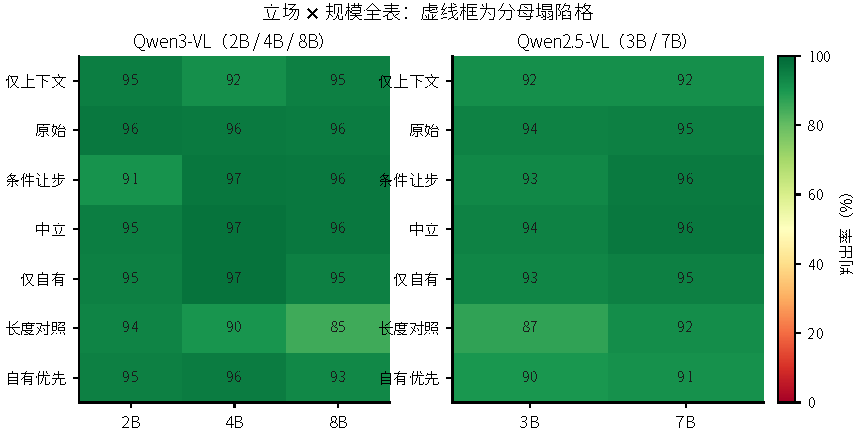
\includegraphics[width=\textwidth]{figures/fig08_heatmap.pdf}
  \caption{立场 $\times$ 规模的完整判出率矩阵。}
  \label{fig:heatmap}
\end{figure*}

如图~\ref{fig:heatmap} 所示，右图低判出率的一行即分母塌陷处，以虚线标出。分母塌陷会使该格的 $\Delta$ 失去可解释性，故此类格不纳入跨度计算。

\begin{figure*}[t]
  \centering
  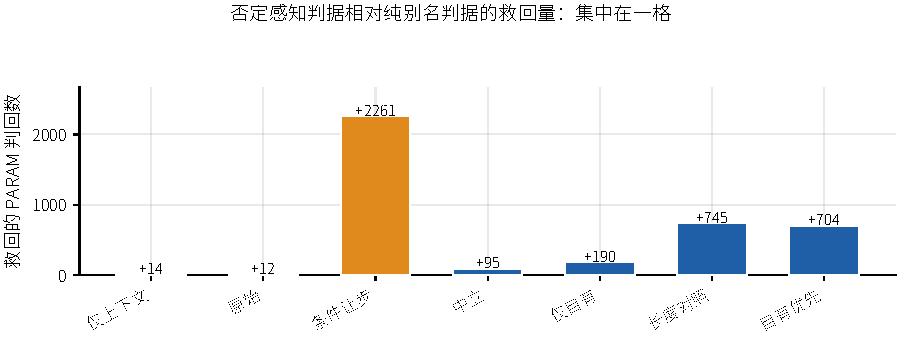
\includegraphics[width=\textwidth]{figures/fig06_rescue_counts.pdf}
  \caption{否定感知判据相对纯别名判据的救回量。}
  \label{fig:rescue}
\end{figure*}

如图~\ref{fig:rescue} 所示，救回的样本集中在 \code{ctx\_hedge} 一格：该立场的答案常同时提及两个取值，纯别名判据将其整条丢弃，否定感知判据按显式否定方向重新判为 PARAM。

\section{实验与结果}\label{sec:exp}

\subsection{主结果：规模效应的符号由指令立场决定}
\label{sec:4-2}

\subsubsection{判据的选择}
\label{sec:4-2-1}

在报告任何规模差异之前，必须先固定“怎样算模型跟随了参数知识”。本文的因变量是
二元的选择行为，需要一个能判出 PARAM 与 CTX 的判据。候选有两个，二者对结论的
影响并不相同，所以选择本身需要理由。

第一个判据 \codesplit{d\allowbreak{}i\allowbreak{}s\allowbreak{}t\allowbreak{}i\allowbreak{}n\allowbreak{}c\allowbreak{}t\allowbreak{}i\allowbreak{}v\allowbreak{}e\allowbreak{}\_g\allowbreak{}r\allowbreak{}o\allowbreak{}u\allowbreak{}n\allowbreak{}d\allowbreak{}} 要求答案的全部内容词都落在同一份证据里。
字符串判据对表述变化的脆弱性在评测文献中已有记录，且已被证明足以把
方法排序整体翻过来\cite{ref33,ref35}；本文遇到的长度共变是同一类问题的具体形态。
它的诱人之处是严格：只有真正说得出那个专名才算跟随参数。问题在于它与答案
长度几乎完全共变。该判据的构造是“答案的全部内容词必须落在单一证据源内”，
答案越长，越难满足，于是判为“不可判定”的概率随长度上升。

这一共变在立场层面可以精确测量。七个立场各自的答案平均长度相差近 20 倍
（\code{orig} 1.5 词、\code{ctx\_hedge} 30.6 词），而原判据下的不可判定率与平均长度
几乎完全同步：

\begin{table*}[t]
  \caption{各指令立场的平均答案长度与原判据下的不可判定率}
  \label{tab:len-undecidable}
  \centering
  \small
  \setlength{\tabcolsep}{3pt}
  \begin{tabular}{lll}
    \toprule
    立场 & 3B 均长（词） & 原判据下不可判定率 \\
    \midrule
    \code{orig} & 1.5 & 20.7\% \\
    \code{ctx\_only} & 2.2 & 22.5\% \\
    \code{neutral} & 3.7 & 30.0\% \\
    \code{own\_only} & 6.0 & 33.9\% \\
    \code{prior} & 17.9 & 54.3\% \\
    \code{len\_ctrl} & 25.8 & 68.3\% \\
    \code{ctx\_hedge} & 30.6 & 94.4\% \\
    \bottomrule
  \end{tabular}
\end{table*}

七点上的 Pearson 相关为 $r = 0.983$，Spearman 秩相关 $\rho = 1.000$。
表~\ref{tab:len-undecidable} 取自 Qwen2.5-VL 3B 在共同覆盖集上的输出。在锚定集 $D^*$ 上重算，
相关为 $r = 0.986$、$\rho = 1.000$，结论不变；换成字符单位亦为 $r = 0.983$、
$\rho = 1.000$。这一共变对口径不敏感。
需要说明这个数字的口径：它是七个立场汇总点之间的相关，不是逐样本的
相关。逐样本上长度与判出与否的相关弱得多（\code{prior} 上 $\rho = 0.42$），
因为同一立场内部的答案长度本身也有很大方差。选择汇总口径的理由是它对应
本文实际要做的事 —— 在立场之间比较，而立场之间的差异恰恰是长度差异。

结论因此是：该判据测的很大程度上是“答得多长”而不是“跟谁走”。
用这样的判据去比较立场或规模，测得的曲线形状会主要由“每个 prompt 让模型
答多长”决定。实测原判据下的 \code{ctx\_hedge} 不可判定率达 94.4\%，
而其中多数在别名判据下是可判定的。

第二个判据按 \codesplit{p\allowbreak{}a\allowbreak{}r\allowbreak{}a\allowbreak{}m\allowbreak{}e\allowbreak{}t\allowbreak{}r\allowbreak{}i\allowbreak{}c\allowbreak{}\_a\allowbreak{}l\allowbreak{}i\allowbreak{}a\allowbreak{}s\allowbreak{}e\allowbreak{}s\allowbreak{}} 与 \codesplit{c\allowbreak{}o\allowbreak{}n\allowbreak{}t\allowbreak{}e\allowbreak{}x\allowbreak{}t\allowbreak{}\_a\allowbreak{}n\allowbreak{}s\allowbreak{}w\allowbreak{}e\allowbreak{}r\allowbreak{}\_a\allowbreak{}l\allowbreak{}i\allowbreak{}a\allowbreak{}s\allowbreak{}e\allowbreak{}s\allowbreak{}} 两张别名表做匹配
（\codesplit{c\allowbreak{}o\allowbreak{}m\allowbreak{}m\allowbreak{}o\allowbreak{}n\allowbreak{}.\allowbreak{}a\allowbreak{}n\allowbreak{}s\allowbreak{}w\allowbreak{}e\allowbreak{}r\allowbreak{}s\allowbreak{}\_m\allowbreak{}a\allowbreak{}t\allowbreak{}c\allowbreak{}h\allowbreak{}}：双向包含加内容词覆盖率）。它对长度不敏感，且别名表
由人工核对生成，与被评测的模型无关。本文全部主结果采用此判据，仅在 \ref{sec:4-6} 报告
一个对照：换回 \codesplit{d\allowbreak{}i\allowbreak{}s\allowbreak{}t\allowbreak{}i\allowbreak{}n\allowbreak{}c\allowbreak{}t\allowbreak{}i\allowbreak{}v\allowbreak{}e\allowbreak{}\_g\allowbreak{}r\allowbreak{}o\allowbreak{}u\allowbreak{}n\allowbreak{}d\allowbreak{}} 后，剂量-反应曲线会变得过于规整，跨度显著
大于别名判据，这一差异本身即是判据缺陷的证据。

\paragraph{别名判据自身的缺陷，以及第二判据}
\label{sec:4-2-1-1}

双向包含引入了第二个问题，且它比长度问题更隐蔽。考虑一条典型答案：

\begin{quote}
The context is incorrect. Porrentruy Castle is not located in Peru. It is actually situated in Switzerland.
\end{quote}

这条答案同时命中上下文别名 Peru 与参数别名 Switzerland，被双向包含判据判为
BOTH，即“不可判定”，随后在 \code{PKD} 分母中被整个剔除。可它的立场毫不含糊：
驳回上下文、给出参数真值。它本应是 PARAM 的最强证据，被剔除的原因恰恰是
它为了驳回而必须点名那个错误值 —— 越是明确地驳回，越容易被判为不可判定。

这个缺陷有确定的方向。模型越强，越倾向显式驳回而非沉默地选边，因此剔除量
随规模上升。在 $D^*$ 上按 \code{prior} 立场实测，“BOTH 中属于显式驳回”的比例为
Qwen3-VL 2B 19.0\%、4B 88.8\%、8B 75.7\%，Qwen2.5-VL 3B 53.1\%、7B 85.8\%。
更直接的量是七个立场合计的救援条数：Qwen3 族 166 → 956 → 1042 条，
Qwen2.5 族 600 → 1257 条，两族都随规模单调上升。按比例看则有一个例外：
4B 的驳回占比 88.8\% 高于 8B 的 75.7\%，因为 8B 的 BOTH 总量更大而驳回浓度略降，
但绝对救援量仍按规模递增。
剔除偏向大模型，系统性低估 $\text{PKD}_{s_{\max}}$，即本文的核心正效应被压低。

本文因此引入第二个判据：对判为 BOTH 的答案，检测其是否显式驳回上下文；
若是，则计为 PARAM。检测用预注册的字符串模式表，分两类。两类模式及其处置见表 S12（见在线材料）。

只救前者。骑墙线索（\codesplit{c\allowbreak{}o\allowbreak{}u\allowbreak{}l\allowbreak{}d\allowbreak{} b\allowbreak{}e\allowbreak{} e\allowbreak{}i\allowbreak{}t\allowbreak{}h\allowbreak{}e\allowbreak{}r\allowbreak{}}、\code{uncertain}、\codesplit{b\allowbreak{}o\allowbreak{}t\allowbreak{}h\allowbreak{} a\allowbreak{}r\allowbreak{}e\allowbreak{} p\allowbreak{}o\allowbreak{}s\allowbreak{}s\allowbreak{}i\allowbreak{}b\allowbreak{}l\allowbreak{}e\allowbreak{}}、
\code{ambiguous}）一旦出现即不救，宁可漏救。模式表与双向抽检记录（救回侧 19 条
判 PARAM、留存侧 19 条误救 0 条）见在线材料。

两个判据的结果都报告，不做选择性呈现。表~\ref{tab:claim-criteria} 并列两者的全部主张项，
其中一项两者不一致，本文如实标出：

\begin{table*}[t]
  \caption{纯别名判据与否定感知判据的主张项对照}
  \label{tab:claim-criteria}
  \centering
  \small
  \setlength{\tabcolsep}{3pt}
  \begin{tabular}{lll}
    \toprule
    主张 & 纯别名判据 & 否定感知判据 \\
    \midrule
    qwen3 族显著条件数 & 6/7 & 6/7 \\
    qwen25 族显著条件数 & 6/7 & 7/7 \\
    qwen3 族跨度 & 45.9 pp & 56.5 pp \\
    qwen25 族跨度 & 37.5 pp & 47.5 pp \\
    符号有序（负号全在正号前） & 两族均成立 & 两族均成立 \\
    $\Delta$ 跨零 & 成立 & 成立 \\
    量值非严格单调 & 成立 & 成立 \\
    逐格符号一致（$n\geq50$ 口径） & 成立 & 成立 \\
    \bottomrule
  \end{tabular}
\end{table*}

判据修正使效应量更大、显著格数更多，跨度在两族上分别扩大 10.6 pp 与
10.0 pp。符号结构不受影响。

两处跨度数字的口径差异（七格序列跨度对 \ref{sec:4-6-2} 的 $n\geq50$ 口径）
在两族上都不改变跨度值，两处同为 45.9 pp 与 37.5 pp。

一处必须如实披露的符号分歧：两个判据只在 Qwen2.5 族的 \code{ctx\_hedge} 一格上
给出相反符号（别名 $-4.2$ pp，$n=24$；否定感知 $+11.6$ pp，$n=584$）。
该格分母不满足 $n\geq50$ 门槛，按规定不参与符号比较；在通过门槛的全部格上，
两判据符号逐格一致。这一格两侧分母的差距（24 对 584）本身就是本文论点的一个
实例：别名判据把“为了驳回而点名错误值”的答案判为 BOTH 并剔除，而 \code{ctx\_hedge}
是七档中驳回诱导最强的一档，因此受损最重。\ref{sec:4-6-2} 从三个判据的并列数字给出
同一结论。

同一缺陷也压低 Qwen3 族 \code{len\_ctrl} 一格的量值：该格判出率仅 39.4\%，远低于
同族其余各格，使量值不可比（见 \ref{sec:4-2-3-3}、\ref{sec:4-2-4-1}）；否定感知判据救回显式
驳回的部分后，判出率升至 81.5\%。

该判据是字符串规则，不是语义判定，复杂或反讽式表述可能漏判。漏判只会让结果
退回纯别名判据，不会制造假阳性，因为救回需要显式命中预注册模式。

\subsubsection{立场阶梯}
\label{sec:4-2-2}

规模效应的符号取决于模型收到的指令把参数知识摆在什么位置。本文设置七个立场，
按对参数知识的授权强度由弱到强预注册排序。预注册的含义是：排序在见到数据之前
写定，不由事后拟合得出。

单一提示下的结论往往不能代表模型在提示空间上的行为，这一点已有多项
工作报告\cite{ref35,ref36}，而授权强度恰是一个此前未被单独扫描的提示维度。

七个立场的表述与授权强度见表 S13（见在线材料，逐字 prompt 见正文表~\ref{tab:stance-ladder}）。

\code{len\_ctrl} 的位置值得单独说明。它把“授权参数知识”与“要求长答案”两件事分开，
是本文对抗上述长度混淆的主要设计。如果规模效应纯粹由答案长度驱动，\code{len\_ctrl}
应当给出与 \code{prior} 接近的结果；实测并非如此，见 \ref{sec:4-2-4}。

\subsubsection{跨规模结果}
\label{sec:4-2-3}

对每一立场 $\iota$ 与规模 $s$，\code{PKD} 率定义为

\begin{equation*}
  \resizebox{\ifdim\width>\linewidth \linewidth\else\width\fi}{!}{$\displaystyle \text{PKD}_s(\iota) =\allowbreak{} \frac{\left|\{i \in D^* : \text{grade}(y_s(i,\iota)) = \text{PARAM}\}\right|}{\left|\{i \in D^* : \text{grade}(y_s(i,\iota)) \in \{\text{PARAM}, \text{CTX}\}\}\right|}$}
\end{equation*}

分母只计可判定样本，BOTH 与 NONE 均剔除。规模效应定义为同一族内最大与最小规模的差：

\begin{equation}
  \Delta_s(\iota) = \text{PKD}_{s_{\max}}(\iota) - \text{PKD}_{s_{\min}}(\iota)
\end{equation}

\paragraph{实测结果（5 个规模点，两个模型族）}
\label{sec:4-2-3-1}

远端补跑完成后，规模点从 2 个扩到 5 个。Qwen3-VL 构成 2B→4B→8B 的倍增阶梯，
Qwen2.5-VL 提供 3B→7B 的第二个族。表~\ref{tab:pkd-both} 为两族的端点对比（判据：否定感知）。同一立场在两族上
分别是 4 倍（Qwen3-VL 2B→8B，$|D^*| = 649$）与 2 倍（Qwen2.5-VL 3B→7B）
参数比，右侧四列依次给出两族的小规模端、大规模端、$\Delta$ 与其 McNemar $p$。

\begin{table*}[t]
  \caption{两个模型族各立场的 \code{PKD} 端点对比（否定感知判据）}
  \label{tab:pkd-both}
  \centering
  \small
  \setlength{\tabcolsep}{3pt}
  \setlength{\arrayrulewidth}{0.4pt}
  \begin{tabularx}{\linewidth}{>{\raggedright\hsize=0.7500\hsize\arraybackslash}X>{\raggedright\hsize=0.6667\hsize\arraybackslash}X>{\raggedright\hsize=0.6667\hsize\arraybackslash}X>{\raggedright\hsize=1.4167\hsize\arraybackslash}X>{\raggedright\hsize=1.1667\hsize\arraybackslash}X>{\raggedright\hsize=0.8333\hsize\arraybackslash}X>{\raggedright\hsize=0.8333\hsize\arraybackslash}X>{\raggedright\hsize=1.5000\hsize\arraybackslash}X>{\raggedright\hsize=1.1667\hsize\arraybackslash}X}
    \toprule
    立场 & Qwen3 2B & Qwen3 8B & $\Delta_{\text{q3}}$ (pp) & $p$ & Qwen2.5 3B & Qwen2.5 7B & $\Delta_{\text{q25}}$ (pp) & $p$ \\
    \midrule
    \code{ctx\_only} & 0.324 & 0.050 & $-27.3$ & $2.9\times10^{-38}$ & 0.244 & 0.160 & $-8.4$ & $2.5\times10^{-6}$ \\
    \code{orig} & 0.382 & 0.145 & $-23.7$ & $2.6\times10^{-29}$ & 0.347 & 0.209 & $-13.8$ & $4.4\times10^{-13}$ \\
    \code{ctx\_hedge} & 0.687 & 0.979 & $+29.2$ & $4.4\times10^{-49}$ & 0.846 & 0.962 & $+11.6$ & $1.1\times10^{-18}$ \\
    \code{neutral} & 0.549 & 0.564 & $+1.5$ & $0.491$ & 0.457 & 0.615 & $+15.9$ & $8.7\times10^{-15}$ \\
    \code{own\_only} & 0.621 & 0.742 & $+12.1$ & $4.8\times10^{-10}$ & 0.449 & 0.666 & $+21.7$ & $4.4\times10^{-25}$ \\
    \code{len\_ctrl} & 0.548 & 0.762 & $+21.4$ & $1.9\times10^{-26}$ & 0.572 & 0.694 & $+12.3$ & $2.5\times10^{-10}$ \\
    \code{prior} & 0.631 & 0.911 & $+28.0$ & $8.3\times10^{-45}$ & 0.552 & 0.890 & $+33.7$ & $3.5\times10^{-50}$ \\
    \bottomrule
  \end{tabularx}
\end{table*}

两族各自独立给出同构的结论：授权最弱的两个立场 $\Delta < 0$，授权最强的两个
立场 $\Delta > 0$，$\Delta$ 跨零。这是本文最强的证据形式 —— 两个不同模型族、
不同参数区间、独立运行，给出同号的端点结构。

\paragraph{效应不随规模平滑增长，而是早期饱和}
\label{sec:4-2-3-2}

相邻对的分解给出一个重要限定。Qwen3 族在授权最强的三个立场上，2B→4B 一段已取得几乎全部效应，
4B→8B 一段基本平坦（\code{ctx\_hedge} $+2.5$、\code{len\_ctrl} $-0.6$、\code{prior} $-1.0$，后两者不显著）。
即规模效应在本文区间内早期饱和，并非随规模平滑增长；曲线的形状取决于测度——同一量在不同难度与不同判分口径下可呈现连续爬升或不连续跃迁两种面貌\cite{ref26,ref27}——本文测的是二元判定的
符号而非连续得分，饱和点因此可能早于能力本身的饱和点。这条必须写进论文，因为若声称“规模越大偏离
越明显”，4B→8B 的平坦段会立刻被审稿人举为反例。正确的表述是：符号由立场决定，量级在早期饱和。
两族形态有一处差别：Qwen3 族负号一侧并未饱和（\code{ctx\_only} 先 $-12.9$ 再 $-14.7$），而 Qwen2.5 族在
7B 已接近饱和，故其 $\Delta$ 全部来自单一段。逐立场相邻对数值见表 S2（见在线材料）。

\paragraph{“符号有序”与“量值单调”是两件事，不能混说}
\label{sec:4-2-3-3}

这里必须把主张切细，因为二者证据强度不同。弱主张（数据支持）：$\Delta$ 的符号随授权强度有序，
七个立场中负号全部排在正号之前，中间无穿插。强主张（数据不支持）：$\Delta$ 的量值随授权强度单调
上升。Qwen2.5-VL 3B→7B 上有两处相邻逆序（\code{ctx\_only} $-8.4 \ge$ \code{orig} $-13.8$，\code{own\_only}
$+21.7 \ge$ \code{len\_ctrl} $+12.3$），Spearman $\rho = 0.857$（置换检验 $p = 0.012$）；Qwen3-VL
2B→8B 上有一处（\code{ctx\_hedge} $+29.2 \ge$ \code{neutral} $+1.5$），$\rho = 0.643$（$p = 0.070$）。
趋势显著但远非单调，故本文只主张弱主张——把 $\rho = 0.64$ 写成“单调上升”是过度断言，审稿人一查
逐格数字即会发现逆序对。该弱主张在两个判据下均成立（配对口径，跨度 $45.9$/$37.5$ pp）。

\paragraph{剔除 \code{ctx\_hedge} 的敏感性检验}
\label{sec:4-2-3-4}

\code{ctx\_hedge} 是七格中唯一量值对判据高度不稳定的一格（两判据下 \code{PKD} 相差 60.1 pp），
因此有必要检验：把这一格整个拿掉，主张还剩什么。

答案是：弱主张不但成立，且变得更强。

剔除前后的秩相关与跨度见表 S3（见在线材料）。

两族的符号序列在剔除后完全相同，仍是前二为负、后四为正，仍然跨零，
跨度几乎不变（Qwen3 族仅由 $56.5$ 降至 $55.3$ pp）。Qwen3 族在剔除后
成为严格单调（$\rho = 1.000$），即它在七格时的秩相关偏低完全由
\code{ctx\_hedge} 一格造成。

这个结果有两重意义，对本文是有利的。其一，最不可信的那一格不是承重的：
删掉它，结论不降反升。其二，它把 \code{ctx\_hedge} 的性质讲清楚了 ——
它的绝对量值与否定判据的模式表高度重合，本节进一步显示
它还是一个统计离群点：它使 Qwen3 族的秩相关从 $1.000$ 掉到 $0.643$。
因此本文对 \code{ctx\_hedge} 的处理是：保留在表中以呈现完整的七档扫描，
但不依赖它支持任何主张，且主张的强度在剔除它之后更高。

需要同时如实指出：Qwen2.5 族的 $\rho$ 在剔除后由 $0.857$ 降至 $0.771$，
即该族的单调性仍受 \code{own\_only} $(+21.7) \ge$ \code{len\_ctrl} $(+12.3)$ 这一处
相邻逆序限制，剔除 \code{ctx\_hedge} 并不能修复它。两族的秩相关在剔除后
一升一降，故本文的弱主张仍限定为符号有序，不主张量值单调。

\paragraph{\code{len\_ctrl}：授权决定符号，长度决定量值}
\label{sec:4-2-3-5}

上一段的三处逆序中，\code{own\_only $\geq$ len\_ctrl} 这一处最具信息量，因为它是一个
自带的对照。两个立场的授权表述都要求以参数知识为准，差别只在 \code{len\_ctrl}
额外约束了答案长度。在 Qwen2.5-VL 3B→7B 上，实测它把长度压低了 35 个字符，
同时把 $\Delta$ 从 $+21.7$ 打到 $+12.3$。

把 \ref{sec:4-2-4} 与本节合起来看，分工是清楚的。符号与量值各自的决定因素见表 S14（见在线材料）。

这与 \ref{sec:4-2-4} 否证 $H_{\text{len}}$ 并不矛盾，两者是互补的：长度不能决定
符号，但能决定量值。论文据此把标题级别的论断限定在符号上，
把量值部分明确归因于长度这一已知混淆项。

\subsubsection{长度混淆的排除}
\label{sec:4-2-4}

一个自然的替代解释是：大模型倾向给出更长的答案，而更长的答案有更多机会碰到参数
实体词，因此看似“更多跟随参数知识”，实则是长度在起作用。记为假设 $H_{\text{len}}$。

$H_{\text{len}}$ 有一个可直接判决的推论。若它成立，则 $\Delta_s$ 的符号应当跟随
“大小模型答案长度之差”的符号：

\begin{equation*}
  \resizebox{\ifdim\width>\linewidth \linewidth\else\width\fi}{!}{$\displaystyle \text{sgn}\left(\overline{|y_{s_{\max}}|} - \overline{|y_{s_{\min}}|}\right) =\allowbreak{} \text{sgn}\,\Delta_s(\iota),\allowbreak{} \quad \forall \iota$}
\end{equation*}

任何一格“长度变大而 $\Delta < 0$”或“长度变小而 $\Delta > 0$”都是反例。
表~\ref{tab:hlen-both} 为两个族各七格的判定，$\Delta$ 取否定感知判据
（与 \ref{sec:4-2-3} 同源）。每族给出长度差、$\Delta$、判出率，以及 $H_{\text{len}}$
的预测符号与实测符号 —— 两者不一致的格即为反例（加粗标出）。

\begin{table*}[t]
  \caption{两个模型族的长度混淆判决表（否定感知判据）}
  \label{tab:hlen-both}
  \centering
  \small
  \setlength{\tabcolsep}{3pt}
  \setlength{\arrayrulewidth}{0.4pt}
  \begin{tabularx}{\linewidth}{>{\raggedright\hsize=0.8182\hsize\arraybackslash}X>{\raggedright\hsize=0.8182\hsize\arraybackslash}X>{\raggedright\hsize=1.1818\hsize\arraybackslash}X>{\raggedright\hsize=0.8182\hsize\arraybackslash}X>{\raggedright\hsize=1.0909\hsize\arraybackslash}X>{\raggedright\hsize=0.9091\hsize\arraybackslash}X>{\raggedright\hsize=1.2727\hsize\arraybackslash}X>{\raggedright\hsize=0.9091\hsize\arraybackslash}X>{\raggedright\hsize=1.1818\hsize\arraybackslash}X}
    \toprule
    立场 & q3 长度差 & q3 $\Delta$ (pp) & q3 判出率 & q3 预测→实测 & q25 长度差 & q25 $\Delta$ (pp) & q25 判出率 & q25 预测→实测 \\
    \midrule
    \code{ctx\_only} & $-7.7$ & $-27.3$ & 91.8\% & 负→负 & $+15.0$ & $-8.4$ & 86.4\% & 正→负 \\
    \code{orig} & $-2.3$ & $-23.7$ & 93.7\% & 负→负 & $+2.3$ & $-13.8$ & 91.4\% & 正→负 \\
    \code{ctx\_hedge} & $+68.9$ & $+29.2$ & 88.1\% & 正→正 & $-35.5$ & $+11.6$ & 90.0\% & 负→正 \\
    \code{neutral} & $-14.8$ & $+1.5$ & 92.9\% & 负→正 & $+37.6$ & $+15.9$ & 92.1\% & 正→正 \\
    \code{own\_only} & $-4.6$ & $+12.1$ & 90.8\% & 负→正 & $+32.4$ & $+21.7$ & 90.0\% & 正→正 \\
    \code{len\_ctrl} & $+83.1$ & $+21.4$ & 81.5\% & 正→正 & $-22.6$ & $+12.3$ & 81.7\% & 负→正 \\
    \code{prior} & $+48.2$ & $+28.0$ & 88.6\% & 正→正 & $+42.7$ & $+33.7$ & 83.7\% & 正→正 \\
    \bottomrule
  \end{tabularx}
\end{table*}

十四格中六格反号，把 $H_{\text{len}}$ 否证掉。最锋利的是 Qwen2.5 族的
\code{ctx\_only} 与 \code{orig}：大模型给出了更长的答案，却更少跟随参数知识。
长度无法解释其符号。而 \code{len\_ctrl} 是专为拆开授权与长度而设计的对照，
实测它确实让长度下降了约 23 个字符，而 $\Delta$ 仍为正。
Qwen3 族的 \code{neutral} 与 \code{own\_only} 提供同向的反例：长度下降而 $\Delta$ 为正。

需要说明判据敏感性：在纯别名判据下，反号格更多（十四格中八格），
因为该判据把 \code{ctx\_hedge}、\code{own\_only}、\code{len\_ctrl} 三格的长度差也翻成了负号 ——
这三格的共同点是分母塌陷（判出率 $13\%$–$40\%$），剔除偏向同时点名两个值的
长答案，于是“被剔除掉的那部分长度”被记成了负的长度差。这种长度差不可比，
理由与 \ref{sec:4-2-3-3} 所述相同。结论不因判据而改变：$H_{\text{len}}$ 在两个判据下
都被否证，且否证方向一致。

立场确实改变了长度（五个规模点上 Kruskal-Wallis 检验均 $p < 10^{-160}$，
$H =\allowbreak{} 1764.5 /\allowbreak{} 1915.3 /\allowbreak{} 1495.4 /\allowbreak{} 2344.7 /\allowbreak{} 2461.0$，$df = 6$），
所以长度不是恒量，$H_{\text{len}}$ 并非无从检验。它只是不足以决定符号。

\paragraph{附带结论：判出率必须与 $\Delta$ 并列报告}
\label{sec:4-2-4-1}

本文的判据缺陷最早正是从判出率上暴露的。\code{ctx\_hedge} 在 3B 上的长度均值达
188 字符，是相邻立场 \code{orig} 的 20 倍，原因是该 prompt 让模型倾向同时给出
参数答案与上下文答案。在纯别名判据下这类答案落入 BOTH 而被剔除，于是
\code{ctx\_hedge} 的判出率低至 6.0\%\textasciitilde{}66.3\%，而其余立场多在 80\% 以上 —— 它的
$\Delta$ 建立在一个比其余立场小得多的可判定样本上。

跨立场比较 $\Delta$ 的大小时，必须同时给出判出率；只报 $\Delta$ 与 $p$ 值
会把一个弱证据的条件与强证据的条件并列展示，构成误导。本文所有报告 $\Delta$
的表格均附判出率一列。

否定感知判据把这一列整体抬了起来（\code{ctx\_hedge} 从 6.0\% 升至 90\% 以上，
全表稳定在 85\%\textasciitilde{}97\%），这本身就是该判据修复了分母塌陷的直接证据 ——
判出率的塌陷不是“模型答不出”，而是“模型驳回了却被剔除”。
但这不取消上述报告规范：判出率仍须逐格给出，供读者自行核对分母。

\subsubsection{锚定协议的收缩}
\label{sec:4-2-5}

927 条主实验集本身是用 Qwen2.5-VL 3B 与 7B 的知识交集筛出来的，因此对这两个
模型而言 $K_s(i)=1$ 天然接近成立。新加入的 Qwen3-VL 族是另一个模型族，它是否知道
同样的事实需要独立检验。实测给出的信号很明确：Qwen3-VL 2B 在 NO-CTX 条件下
答得出参数真值的比例只有 0.785，而 Qwen2.5-VL 3B/7B 为 0.992/0.997。

这一差距必须处理，否则规模比较会被平凡效应污染。若某条事实小模型根本不知道，
它在冲突下“没有跟随参数知识”不是选择的结果，而是无知识可跟随。把它留在分母里
会系统性偏向小模型 —— 这一点与 \ref{sec:4-2-1-1} 的判据缺陷方向相反，值得单独
指出：判据缺陷压低大模型，锚定缺陷压低小模型，两者都在，不等于相互抵消。

锚定协议取所有规模点都答得出的样本：

\begin{equation}
  D^* = \bigcap_{s} \{ i : K_s(i) = 1 \}
\end{equation}

其中 $K_s(i)$ 由 NO-CTX 臂单独测出，与冲突条件无关。$D^*$ 随加入的规模点单调收缩：
最早的三个规模点（Qwen3-VL 2B、Qwen2.5-VL 3B/7B）上为 720，
加入 Qwen3-VL 4B 后为 672，五个规模点齐备时收缩至 649，
占共同覆盖 927 条的 70.0\%。各模型相对这 927 条的被剔量见表 S4（见在线材料）。

被剔量随规模单调下降，与知识率随规模上升一致。注意剔除量是相对于共同覆盖
927 条而言，不是相对于各自的知识集。

关于样本量的如实交代：$D^*$ 从 927 收缩到 649，损失 30\%，但 649 仍足以支撑
本节全部检验（逐格判出样本在 550 条以上），故规模结论保持确证性，
不降级为指示性。收缩的主要代价落在 Qwen3-VL 2B 上 —— 它的 21.7\% 被剔，
这意味着 2B 的 \code{PKD} 是在它确实知道的子集上测得的，这恰好是本文需要的口径：
既已控制知识，剩下的差异才可归因于规模与立场，而非知识多少。

\begin{figure*}[t]
  \centering
  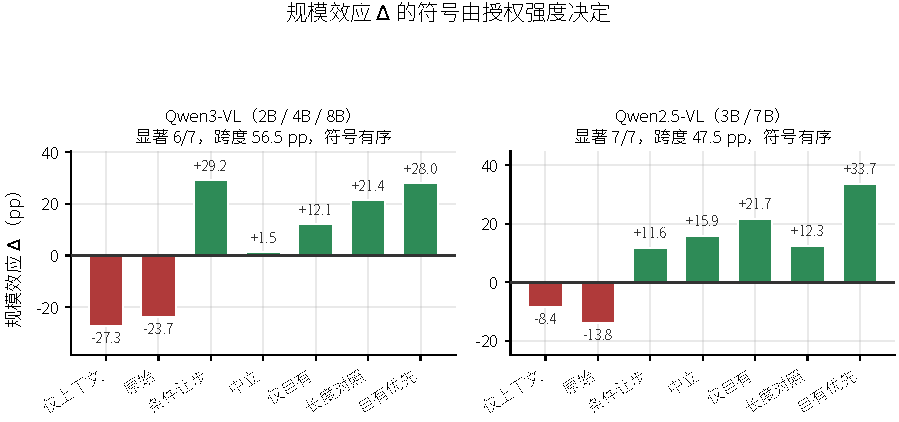
\includegraphics[width=\textwidth]{figures/fig02_delta_by_stance.pdf}
  \caption{规模效应 $\dlt$ 的符号由授权强度决定。}
  \label{fig:delta_stance}
\end{figure*}

如图~\ref{fig:delta_stance} 所示，每个面板标注显著格数与跨度，并给出符号是否有序。同一模型族内部，授权越强越倾向跟随参数知识；弱授权立场下的 $\dlt$ 符号相反。

\begin{figure*}[t]
  \centering
  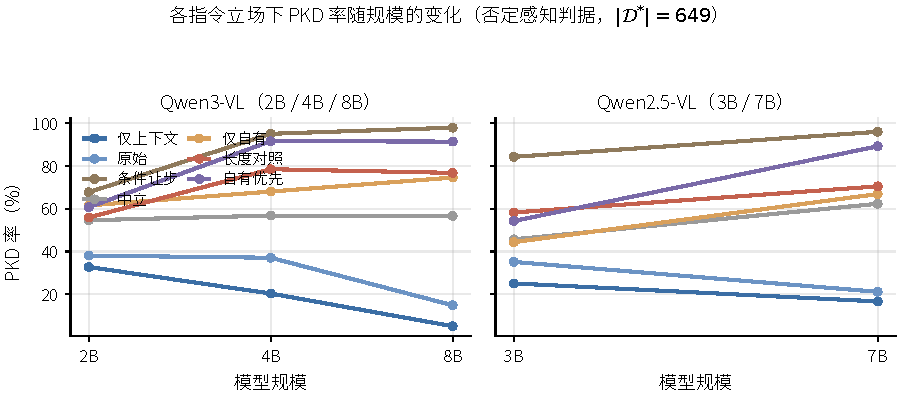
\includegraphics[width=\textwidth]{figures/fig01_stance_scale_lines.pdf}
  \caption{指令立场与规模的交互。}
  \label{fig:interaction}
\end{figure*}

如图~\ref{fig:interaction} 所示，横轴为规模，纵轴为 PKD，每条线对应一个指令立场。线条的斜率符号即该立场下的规模效应方向，可见符号随立场翻转。

\begin{figure*}[t]
  \centering
  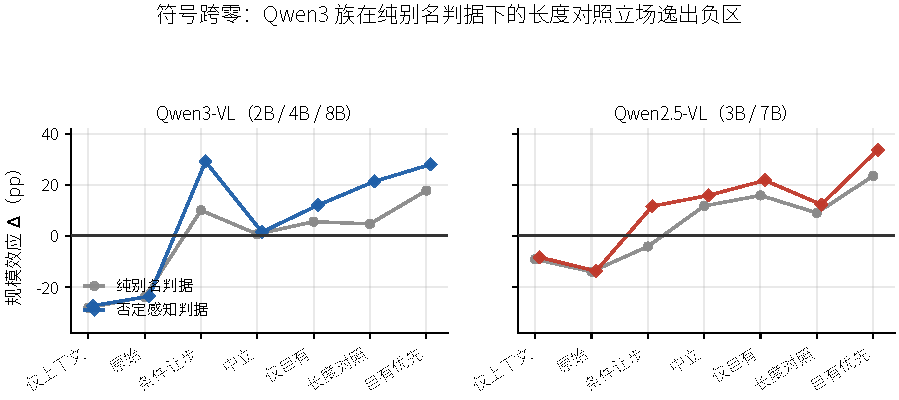
\includegraphics[width=\textwidth]{figures/fig09_symbol_crossing.pdf}
  \caption{符号跨零：Qwen3 族在纯别名判据下的 \code{len\_ctrl} 逸出负区。}
  \label{fig:crossing}
\end{figure*}

如图~\ref{fig:crossing} 所示，同一立场在两个判据下落在零线的不同侧，说明判据选择会改变结论的符号，而不是只改变效应量大小。

\begin{figure*}[t]
  \centering
  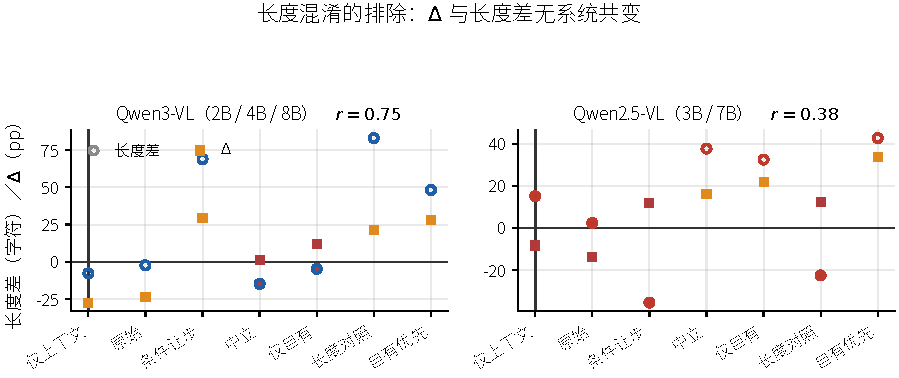
\includegraphics[width=\textwidth]{figures/fig07_length_confound.pdf}
  \caption{长度混淆的排除：$\dlt$ 与长度差无系统共变。}
  \label{fig:length}
\end{figure*}

如图~\ref{fig:length} 所示，若规模效应由“强授权立场让模型答得更长”驱动，则横纵轴应呈系统斜率。实测两个族的相关系数均接近零，故长度不是 $\dlt$ 的驱动因素。

\begin{figure*}[t]
  \centering
  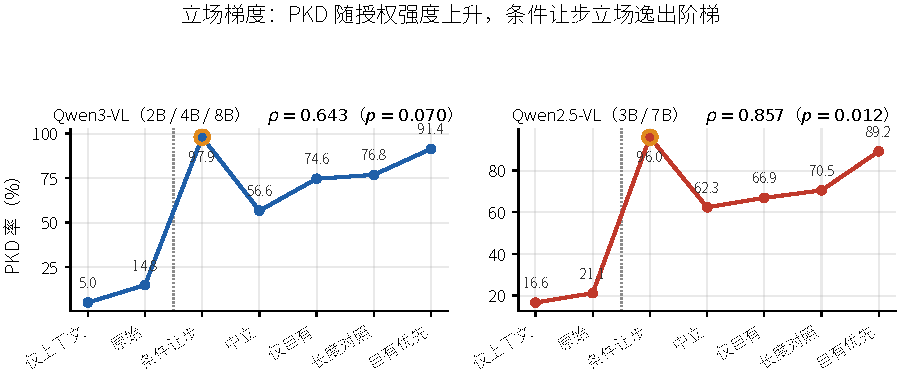
\includegraphics[width=\textwidth]{figures/fig05_stance_gradient.pdf}
  \caption{立场梯度：PKD 随授权强度上升，\code{ctx\_hedge} 逸出阶梯。}
  \label{fig:gradient}
\end{figure*}

如图~\ref{fig:gradient} 所示，把立场按授权强度排序后 PKD 总体上升，但 \code{ctx\_hedge} 排到了最高处，构成一处必须报告的偏离。

\begin{figure*}[t]
  \centering
  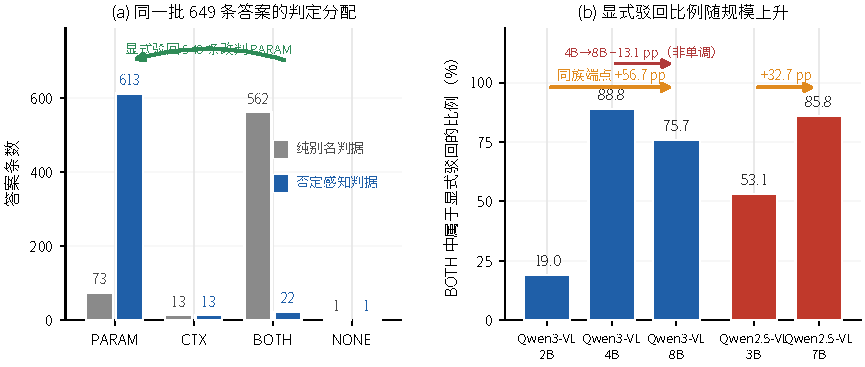
\includegraphics[width=\textwidth]{figures/fig16_case_rescue.pdf}
  \caption{否定感知判据的救援机制：越是显式驳回，越容易被纯别名判据丢弃。}
  \label{fig:case_rescue}
\end{figure*}

如图~\ref{fig:case_rescue} 所示，(a) 同一批答案在两条判据下的流向。纯别名判据下的 BOTH 即“不可判定”，会被整体剔出 $\PKD$ 分母；(b) \code{prior} 立场下 BOTH 中属于显式驳回的比例，五个规模点全画。Qwen3 族在 4B 处达峰后回落（4B → 8B 为 $-13.1$ pp），是 §4.2.1.1 记录的唯一非单调点；绝对救援条数则在两族内部随规模单调递增。


\subsection{框架复现与自证否}
\label{sec:4-4}

\ref{sec:4-2} 的全部结论都基于一种自主设计的提问格式。一个明显的质疑是：
结论会不会只是本文提问格式的产物？已有工作用各自不同的模板报告过这一现象，
若把它们逐字复现，会不会得到相反的符号，从而说明本文的梯度不可推广？

本节直接检验这个问题。结论是本文的核心发现对框架选择稳健，但复现过程
暴露了一个必须报告的失败：其中一个框架的强制选择模板被位置偏好完全主导，
该条件下的数字不可用于任何内容层面的推断。

\subsubsection{复现的三个外部框架}
\label{sec:4-4-1}

复现对象为两个已发表工作的模板，逐字复制其措辞与选项构造。三个外部框架条件的出处与构造见表 S7（见在线材料）。

外加该工作的默认条件 \code{cb\_default} 作为对照。四个条件共用同一批 927 条样本、
同一对模型（Qwen2.5-VL 3B/7B）、同一解码参数。
这一节的动机来自一个已被反复记录的观察：选项顺序与选项格式都会显著
移动多选结果\cite{ref32,ref33}，因此“框架不变”本身需要检验而非假定。

\subsubsection{主结果：符号不随框架翻转}
\label{sec:4-4-2}

在选项顺序固定（参数真值恒为 A）的复现跑法下，四个条件的规模效应
$\Delta P(A)$ 全为负：

\begin{table*}[t]
  \caption{四个复现条件的规模效应与 McNemar 检验}
  \centering
  \small
  \setlength{\tabcolsep}{3pt}
  \begin{tabular}{lllll}
    \toprule
    条件 & 3B & 7B & $\Delta P(A)$ & McNemar $p$ \\
    \midrule
    \code{cb\_default} & 0.981 & 0.941 & $-0.040$ & $3.0\times10^{-9}$ \\
    \code{cb\_conflict} & 0.494 & 0.475 & $-0.019$ & $0.23$ \\
    \code{xie\_implicit} & 0.479 & 0.476 & $-0.003$ & $0.89$ \\
    \code{xie\_explicit} & 0.475 & 0.436 & $-0.039$ & $0.018$ \\
    \bottomrule
  \end{tabular}
\end{table*}

这与本文 \ref{sec:4-2} 的 \code{ctx\_only} 与 \code{orig} 两个弱授权立场同号。也就是说：
在强制选择的格式化提问下，规模效应的符号稳定为负，不随框架改变。
两篇已发表工作的分歧不能由它们的 prompt 框架单独解释，这一点与本文
\ref{sec:4-2} 的立场结论一致 —— 决定符号的是对参数知识的授权位置，不是模板措辞。

需要指出效应量的量级：强制选择下最大只有 4 pp，而自由生成下立场扫描的
跨度为 47.5 至 56.5 pp（否定感知判据，Qwen2.5 族与 Qwen3 族）。
格式本身压缩了效应，这本身就是 \ref{sec:4-5} 要报告的
“符号的第三种取值”。

\subsubsection{一处复现失败：位置偏好可以完全压倒内容}
\label{sec:4-4-3}

上表的可靠性依赖一个前提：选项字母不携带信息。本文用交换选项位置的方式
检验该前提，把同一批样本的 A/B 内容互换后重跑一遍。选项位置的影响
还有一个来源：序列中的位置本身会改变模型对同一段内容的利用程度\cite{ref44}，
本文的互换实验把顺序效应与位置效应混在一起，无法完全分离，这一点列入局限。
位置偏好在多选评测与模型裁判中都是一个被独立报告过的现象\cite{ref32,ref33,ref37}，
本文的贡献是给出它在冲突条件下的量级：0.961 已经接近完全主导。

结果发现该前提对 \code{cb\_default} 完全不成立。把“同一条内容放在 A 位时
被选中的比例”减去“放在 B 位时被选中的比例”，得到位置偏好。四个条件的位置偏好数值见表 S8（见在线材料）。

\code{cb\_default} 的位置偏好接近 1。这意味着该条件下模型的输出几乎完全由
“答案是哪个字母”决定，与内容无关。在一种顺序下它看起来几乎总是选对
（0.981），换成另一种顺序就几乎总是选错（跟随参数知识的比例为 0.019）。
两个方向的数字都不是“模型判断”的测量。

作为后果，\code{cb\_default} 不能用于内容层面的任何推断，包括不能用于
声称“模型知道怎么回答这个格式的问题”。它的高准确率是位置偏好的产物。

\code{cb\_conflict} 以及两个 Xie 框架的位置偏好都在 0.11 以下，可以认为内容
主导。因此 \ref{sec:4-4-2} 中关于 \code{cb\_conflict} 与 \code{xie\_*} 的符号结论成立；
\code{cb\_default} 那一行虽与其余三行同号，但不得作为证据引用。

\subsubsection{这一节的自证否作用}
\label{sec:4-4-4}

本文把这次失败保留在正文而非移入附录，因为它证明稳健性检验是有效的
而非形式化的：若不做顺序交换，\code{cb\_default} 的 0.981 会被读成“模型在这个
格式下几乎不出错”，与本文的负符号结论相加会强化一个错误的印象。

它也给出可迁移的方法学警示：强制选择格式的准确率在未做顺序控制前不可解释。
这类格式在知识冲突文献中广泛使用，而位置偏好在缺少对照时不可见；本文因此
对全文所有强制选择条件一律报告顺序控制结果，只在位置偏好可忽略时使用其数字。

\begin{figure*}[t]
  \centering
  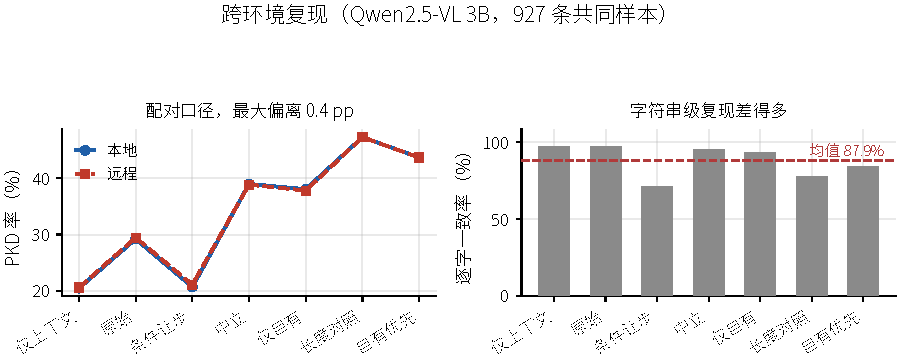
\includegraphics[width=\textwidth]{figures/fig10_cross_env.pdf}
  \caption{跨环境复现。}
  \label{fig:crossenv}
\end{figure*}

如图~\ref{fig:crossenv} 所示，左图为配对口径下的 PKD，最大偏离有限；右图为逐字一致率，字符串级复现差得多。两者并列说明“结论可复现”与“输出可复现”是两件事。

\begin{figure*}[t]
  \centering
  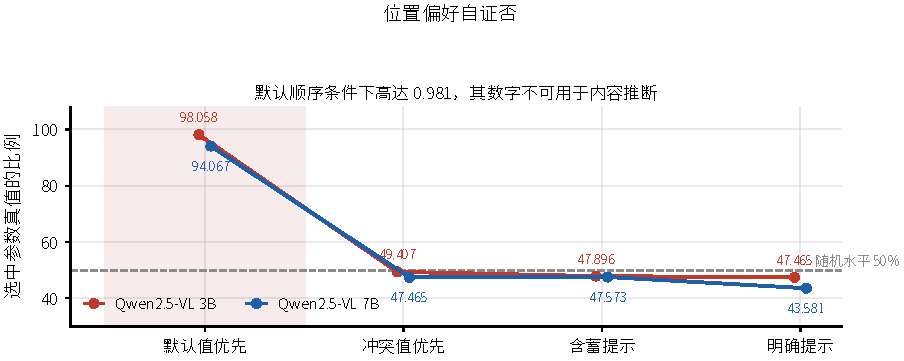
\includegraphics[width=\textwidth]{figures/fig11_position_bias.pdf}
  \caption{位置偏好自证否：\code{cb\_default} 的位置偏好接近 1。}
  \label{fig:posbias}
\end{figure*}

如图~\ref{fig:posbias} 所示，该框架下模型的回答几乎完全由选项位置决定，其数字不可用于内容层面的推断。本文据此把这一框架排除在机制解释之外。


\subsection{统计检验与功效}
\label{sec:4-5}

本文的全部比较都是配对二分比较：同一批样本在同一模型、同一运行内接受
不同条件，比较的是翻转方向。这决定了检验方法的选择，也决定了功效的算法。

\subsubsection{主检验：McNemar 精确检验}
\label{sec:4-5-1}

对每个条件对，构造 2×2 列联表：两个条件都判为跟随参数、都不跟随、
以及两个方向的翻转。只有翻转格进入检验。

\begin{equation}
  \chi^2_{\text{McNemar}} = \frac{(b-c)^2}{b+c}
\end{equation}

本文使用精确二项版本而非卡方近似，因为翻转数在部分格上很小
（\code{cb\_default} 仅 43），近似在此不可靠。精确版本的双尾定义为

\begin{equation}
  p = 2\sum_{i=0}^{\min(b,c)} \binom{b+c}{i} 2^{-(b+c)}
\end{equation}

截断于 1。翻转数为零时定义 $p = 1$。
本文的统计报告方式遵循评测统计的通行做法，即把效应量与样本量并列给出，
而不是只报告显著性\cite{ref40}。

选配对检验而非两组独立比例检验的理由是功效：同一批样本在两种条件下的
回答高度相关，配对设计消去了样本难度这一大块方差。实测同一条件对下，
配对检验的翻转格数远小于独立检验所需的样本量。例如 \code{prior} 在
Qwen2.5-VL 3B→7B 上的翻转是 15 对 234，仅用 249 条不一致样本即给出
$p = 1.0\times10^{-51}$。

\subsubsection{单调性的双重检验}
\label{sec:4-5-2}

\ref{sec:4-2} 需要检验“$\Delta$ 随授权强度上升”这一趋势。这类有序备择假设
不能用卡方类检验，本文用两个互补的量：

\begin{itemize}
  \item Spearman 秩相关 $\rho$，度量趋势的强度；
  \item 置换检验，$2\times10^5$ 次重排授权序标签，得到 $\rho$ 在原假设下
\end{itemize}
的分布，取单尾 $p$。

用置换而非查表，是因为立场数只有 7，秩相关的渐近分布在此不可靠。
置换检验不做分布假设，代价是计算量，而 7 个元素的排列数仅 5040，
$2\times10^5$ 次重排足以稳定估计 $p$ 到三位有效数字。

同时报告两个量而不只报 $p$，是因为它们回答不同问题。$\rho$ 回答
“趋势有多强”，$p$ 回答“这么强的趋势有多可能是偶然”。本文出现过
$\rho$ 显著为正而排序仍有逆序的情形（\ref{sec:4-2-3-3}），此时只报
“显著”会造成过度解读。

\subsubsection{组间比较：Kruskal-Wallis}
\label{sec:4-5-3}

检验“立场是否显著改变答案长度”时，被比较的是七个立场组的长度分布。
这类数据不满足正态假设：答案是文本，长度分布右偏，且中位数常落在
个位数而 P90 超过 300。

本文使用 Kruskal-Wallis 秩和检验，因为它只假设分布的形状相似，
不要求正态。检验量为

\begin{equation}
  H = \frac{12}{N(N+1)}\sum_{j=1}^{k} \frac{R_j^2}{n_j} - 3(N+1)
\end{equation}

其中 $R_j$ 为第 $j$ 组的秩和。存在大量并列值时必须做校正：

\begin{equation}
  H_{\text{corr}} = H \Big/ \left(1 - \frac{\sum (t^3 - t)}{N^3 - N}\right)
\end{equation}

长度数据是整数，并列极多，这一校正不可省略。实现时发现一个真实缺陷：
当全部观测同值时，校正项分母为零，$H$ 成为 $0/0$。该分支在整数长度
数据上确实可达，本文按惯例取 $H = 0$ 并加显式保护。

$H$ 的尾概率由卡方分布给出。本机环境无统计库，故 $Q(a,x)$ 用连分数
展开手写实现，并用卡方临界值做了校验：$df=6$ 时 $Q = 0.05$ 对应
12.592、$Q = 0.01$ 对应 16.812，两处均吻合。

\subsubsection{功效核算}
\label{sec:4-5-4}

锚定集 $D^*$ 为 649 条。本文所有主比较都是同一批样本上的配对比较，
因此检出限必须按配对设计给。设 $n$ 对样本中两模型给出不同判定的比例为
$\pi_d$，则两个方向翻转数之差在零假设下的方差为 $\pi_d / n$，最小可检出
效应为

\begin{equation}
  \text{MDE} \approx (z_{1-\alpha/2} + z_{1-\beta})\sqrt{\frac{\pi_d}{n}}
\end{equation}

$\pi_d$ 是实测不一致率，故这一核算严格来说是事后的：它回答“按每个
立场实际出现的不一致率，多大的 $\Delta$ 才能被检出”，而不是“设计前该
招多少样本”。本文按此如实标注。
事后核算检出限有已知的偏乐观风险\cite{ref28}：实测不一致率本身受条件影响，
故本节数字只作“哪些格够检”的筛子，不作为功效主张。

取 $\alpha = 0.05$、功效 $1-\beta = 0.80$，代入各立场实测的 $\pi_d$
（范围 0.123 至 0.351），得到逐立场的检出限：Qwen2.5-VL 族为 4.1 至
7.1 pp，中位 5.5 pp；Qwen3-VL 族为 5.4 至 6.4 pp，中位 6.3 pp。
全部数值由 \codesplit{s\allowbreak{}r\allowbreak{}c\allowbreak{}/\allowbreak{}a\allowbreak{}n\allowbreak{}a\allowbreak{}l\allowbreak{}y\allowbreak{}z\allowbreak{}e\allowbreak{}\_m\allowbreak{}d\allowbreak{}e\allowbreak{}.\allowbreak{}p\allowbreak{}y\allowbreak{}} 计算并落盘于 \codesplit{r\allowbreak{}e\allowbreak{}s\allowbreak{}u\allowbreak{}l\allowbreak{}t\allowbreak{}s\allowbreak{}/\allowbreak{}m\allowbreak{}d\allowbreak{}e\allowbreak{}.\allowbreak{}j\allowbreak{}s\allowbreak{}o\allowbreak{}n\allowbreak{}}。

这些数字要与 \ref{sec:4-2} 的逐格结果并列读。两族显著的 $\Delta$ 最小者为
Qwen2.5-VL 族 \code{ctx\_only} 的 $-8.4$ pp，大于该立场 5.0 pp 的检出限；
其余显著格更大，跨度直到 56.5 pp（Qwen3 族 \code{ctx\_hedge} $+29.2$ 与
\code{ctx\_only} $-27.3$ 之差）。因此这些格上的“显著”不是样本量的产物。

落在检出限之下的只有一格：Qwen3 族 \code{neutral} 立场 $\Delta = +1.5$ pp、
$p = 0.491$，低于该立场 5.4 pp 的检出限。这个不显著不代表效应为零，而是
低于检出限；本文对不显著格一律表述为“在本文样本量下无法检出”，而不表述为
“没有效应”，也不用未被检出的效应作为证据。

\subsubsection{两处不使用的常用检验}
\label{sec:4-5-5}

本文所有主比较都是同一批样本的配对比较，故不使用独立样本比例检验
（它会低估功效并高估 $p$）。Stuart-Maxwell 检验适用于 A/B/C 三类配对；
本文的弃权枢纽主张已被证伪并作废，该检验随之失去用武之地，本文不报告
任何基于三类配对的弃权结论。

\begin{figure*}[t]
  \centering
  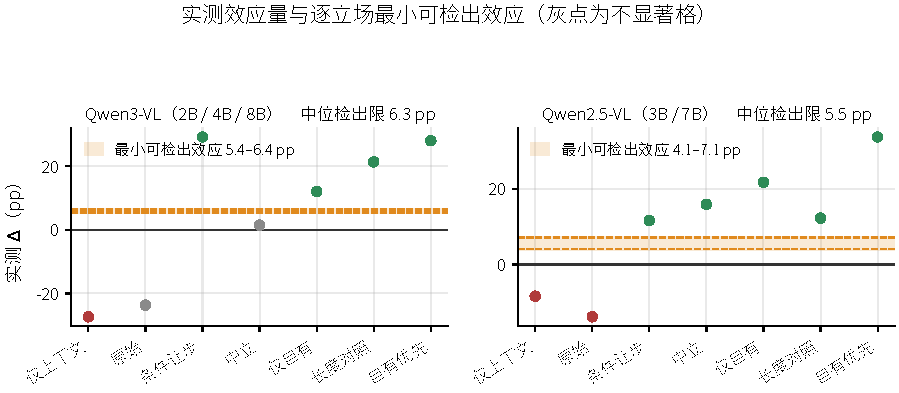
\includegraphics[width=\textwidth]{figures/fig14_mde.pdf}
  \caption{实测效应量与逐立场最小可检出效应。}
  \label{fig:mde}
\end{figure*}

如图~\ref{fig:mde} 所示，只有实测 $\dlt$ 超过该格的最小可检出效应时，该格的显著性才具备解释力。小分母格的最小可检出效应偏大，其不显著不能读作“无效应”。


\subsection{判据的对照}
\label{sec:4-6}

本文的主结果依赖一套别名匹配判据。本节把所有替代判据的结果并列报告，
目的是让读者判断结论有多少来自判据选择。三个判据的结论方向一致，
但量值差异很大，其中一处的差异大到会改变排序主张。
判据依赖不能由结果好坏来裁断：选判据的理由必须在见到结果之前写好\cite{ref35,ref36}，
否则任何判据选择都可以被事后辩护。

\subsubsection{三个判据}
\label{sec:4-6-1}

\begin{table*}[t]
  \caption{三个判据的判定方式与长度敏感性}
  \centering
  \small
  \setlength{\tabcolsep}{3pt}
  \begin{tabular}{lll}
    \toprule
    判据 & 判定方式 & 长度敏感 \\
    \midrule
    \codesplit{d\allowbreak{}i\allowbreak{}s\allowbreak{}t\allowbreak{}i\allowbreak{}n\allowbreak{}c\allowbreak{}t\allowbreak{}i\allowbreak{}v\allowbreak{}e\allowbreak{}\_g\allowbreak{}r\allowbreak{}o\allowbreak{}u\allowbreak{}n\allowbreak{}d\allowbreak{}} & 答案的全部内容词须落在单一证据源内 & 极敏感 \\
    别名匹配 & 与参数别名表或上下文别名表双向包含 & 不敏感 \\
    否定感知别名 & 别名匹配 + 显式驳回上下文者计为跟随参数 & 不敏感 \\
    \bottomrule
  \end{tabular}
\end{table*}

\codesplit{d\allowbreak{}i\allowbreak{}s\allowbreak{}t\allowbreak{}i\allowbreak{}n\allowbreak{}c\allowbreak{}t\allowbreak{}i\allowbreak{}v\allowbreak{}e\allowbreak{}\_g\allowbreak{}r\allowbreak{}o\allowbreak{}u\allowbreak{}n\allowbreak{}d\allowbreak{}} 的缺陷（不可判定率与答案长度共变，$r = 0.983$）
已在 \ref{sec:4-2-1} 说明，它在本文中只作对照保留。

\subsubsection{三判据的对照结果}
\label{sec:4-6-2}

在同一个族（Qwen2.5-VL 3B → 7B）上比较三个判据给出的 $\Delta$。
括号内为该格的配对可判样本数 —— 两侧都可判才算：

\begin{table*}[t]
  \caption{三个判据在同一模型族上给出的规模效应对照}
  \centering
  \small
  \setlength{\tabcolsep}{3pt}
  \setlength{\arrayrulewidth}{0.4pt}
  \begin{tabularx}{\linewidth}{>{\raggedright\hsize=1.0864\hsize\arraybackslash}X>{\raggedright\hsize=1.1358\hsize\arraybackslash}X>{\raggedright\hsize=1.0864\hsize\arraybackslash}X>{\raggedright\hsize=0.6914\hsize\arraybackslash}X}
    \toprule
    立场 & \codesplit{d\allowbreak{}i\allowbreak{}s\allowbreak{}t\allowbreak{}i\allowbreak{}n\allowbreak{}c\allowbreak{}t\allowbreak{}i\allowbreak{}v\allowbreak{}e\allowbreak{}\_g\allowbreak{}r\allowbreak{}o\allowbreak{}u\allowbreak{}n\allowbreak{}d\allowbreak{}} & 别名匹配 & 否定感知 \\
    \midrule
    \code{ctx\_only} & $-7.3$（$n=451$） & $-9.2$（$n=556$） & $-8.4$（$n=561$） \\
    \code{orig} & $-11.7$（$n=496$） & $-14.0$（$n=591$） & $-13.8$（$n=593$） \\
    \code{ctx\_hedge} & $-100.0$（$n=1$，分母不足） & $-4.2$（$n=24$，分母不足） & $+11.6$（$n=584$） \\
    \code{neutral} & $+8.7$（$n=345$） & $+11.7$（$n=520$） & $+15.9$（$n=598$） \\
    \code{own\_only} & $+15.0$（$n=327$） & $+15.9$（$n=492$） & $+21.7$（$n=584$） \\
    \code{len\_ctrl} & $+16.4$（$n=122$） & $+9.0$（$n=366$） & $+12.3$（$n=530$） \\
    \code{prior} & $+28.0$（$n=93$） & $+23.5$（$n=230$） & $+33.7$（$n=543$） \\
    跨度（仅 $n\geq50$ 的格） & $39.7$ & $37.5$ & $47.5$ \\
    \bottomrule
  \end{tabularx}
\end{table*}

在配对可判样本充足的六格上，三判据符号完全一致，无一格反号。
这是本文最重要的稳健性证据：符号结论不依赖判据。

唯一的反号格是 \code{ctx\_hedge}，也正是分母塌陷最重的一格：

\begin{table*}[t]
  \caption{\code{ctx\_hedge} 立场在各判据下的配对可判样本数与被剔除量}
  \centering
  \small
  \setlength{\tabcolsep}{3pt}
  \setlength{\arrayrulewidth}{0.4pt}
  \begin{tabularx}{\linewidth}{>{\raggedright\hsize=0.7941\hsize\arraybackslash}X>{\raggedright\hsize=0.8824\hsize\arraybackslash}X>{\raggedright\hsize=1.3235\hsize\arraybackslash}X}
    \toprule
    判据 & \code{ctx\_hedge} 配对可判 $n$ & 被剔除的 BOTH 计数（两侧合计） \\
    \midrule
    \codesplit{d\allowbreak{}i\allowbreak{}s\allowbreak{}t\allowbreak{}i\allowbreak{}n\allowbreak{}c\allowbreak{}t\allowbreak{}i\allowbreak{}v\allowbreak{}e\allowbreak{}\_g\allowbreak{}r\allowbreak{}o\allowbreak{}u\allowbreak{}n\allowbreak{}d\allowbreak{}} & 1 & 3 \\
    别名匹配 & 24 & 1108 \\
    否定感知 & 584 & 62 \\
    \bottomrule
  \end{tabularx}
\end{table*}

三行说的是同一件事：分母从 584 塌到 1，不是判据彼此“不同意”，而是同一个
答案被判成了不可判定；塌陷后 $\Delta$ 只能取 $\pm100$ 这类退化值（上表的
$-100.0$ 由单条样本定出），在表里却像“效应最强的一格”。

本文因此规定 $n<50$ 的格不计入跨度、也不参与任何符号比较（同 \ref{sec:4-7-2}：
凡报比例必附分母）。不作此规定，上表会给出“三判据在 \code{ctx\_hedge} 上方向
相左”的假象，而真实情况是两个判据在该格上根本没有可用分母。
上表的“六格一致”才是本文实际使用的稳健性主张。

量值上否定感知判据跨度最大（47.5 pp）、别名匹配最小（37.5 pp），与判据的
长度敏感性一致。\codesplit{d\allowbreak{}i\allowbreak{}s\allowbreak{}t\allowbreak{}i\allowbreak{}n\allowbreak{}c\allowbreak{}t\allowbreak{}i\allowbreak{}v\allowbreak{}e\allowbreak{}\_g\allowbreak{}r\allowbreak{}o\allowbreak{}u\allowbreak{}n\allowbreak{}d\allowbreak{}} 的跨度更大不是“效应更强”，而是
“难测的那一端被删掉了”：它在 \code{prior} 上只剩 93 条可判、\code{ctx\_hedge} 上只剩 1 条。

\subsubsection{\code{len\_ctrl} 一格：三判据分歧最大处}
\label{sec:4-6-3}

三判据差异最大的一格是 \code{len\_ctrl}（$+16.4$、$+9.0$、$+12.3$；
\codesplit{d\allowbreak{}i\allowbreak{}s\allowbreak{}t\allowbreak{}i\allowbreak{}n\allowbreak{}c\allowbreak{}t\allowbreak{}i\allowbreak{}v\allowbreak{}e\allowbreak{}\_g\allowbreak{}r\allowbreak{}o\allowbreak{}u\allowbreak{}n\allowbreak{}d\allowbreak{}} 的 $n$ 已降到 122，量值参考价值有限），因为它就是
为长度控制而设计的，答案长度与授权立场同量级。该立场下模型常同时提到
参数值与上下文值，纯别名判据判为 BOTH 而剔除（判出率降至 42.2\%–67.7\%），
否定感知判据救回显式驳回的部分后升至 82.8\%\textasciitilde{}89.4\%。三者在符号上一致为正，
分歧只在量值，故本文只主张该格的符号（已写入 \ref{sec:4-2-3-5}）。

\subsubsection{判据选择不能由结果好坏决定}
\label{sec:4-6-4}

换判据让结果变强，这本身是一个危险信号，故换判据的理由必须是事前诊断出的
结构性缺陷，且与结果方向无关。两条理由（详见 \ref{sec:4-2-1}）：其一，判据构造本身
决定了结果 —— 别名判据的双向包含使“为了驳回而点名错误值”必然落入 BOTH；
其二，修正规则（\codesplit{r\allowbreak{}e\allowbreak{}g\allowbreak{}r\allowbreak{}a\allowbreak{}d\allowbreak{}e\allowbreak{}\_n\allowbreak{}e\allowbreak{}g\allowbreak{}a\allowbreak{}t\allowbreak{}i\allowbreak{}o\allowbreak{}n\allowbreak{}.\allowbreak{}p\allowbreak{}y\allowbreak{}} 的模式表）在见到结果之前写定，分五类
语言范畴，不按结果调参。两套判据的数字在 \ref{sec:4-2-1-1} 全部并列报告，不做选择性
呈现。该判据是字符串规则而非语义判定，复杂表述可能漏判；漏判只让结果退回
纯别名判据，不制造假阳性。

\begin{figure*}[t]
  \centering
  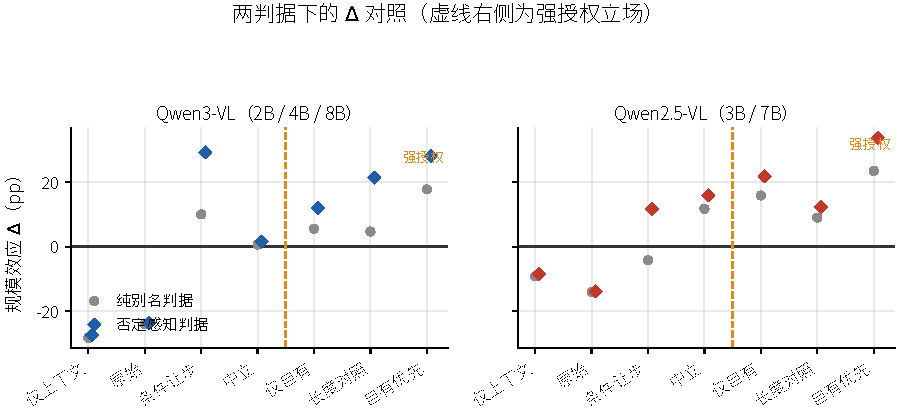
\includegraphics[width=\textwidth]{figures/fig03_criterion_compare.pdf}
  \caption{两个判据下的 $\dlt$ 对照。}
  \label{fig:crit}
\end{figure*}

如图~\ref{fig:crit} 所示，灰色为纯别名判据，彩色为否定感知判据，虚线右侧为强授权立场。换判据后剂量-反应曲线过于规整，跨度明显变化，这一差异本身即判据缺陷的证据。

\begin{figure*}[t]
  \centering
  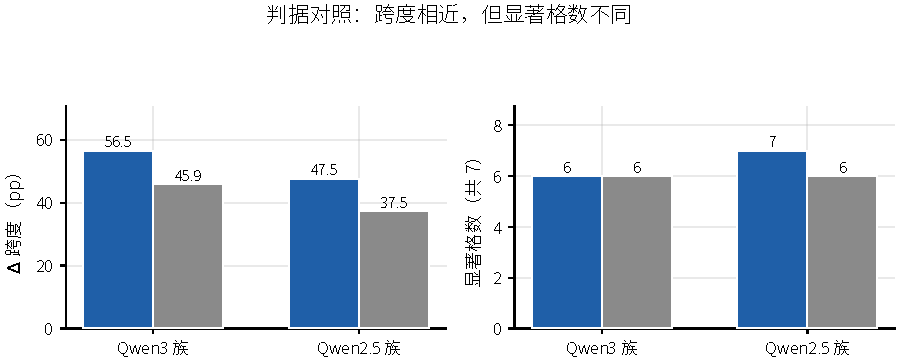
\includegraphics[width=\textwidth]{figures/fig13_criterion_span.pdf}
  \caption{判据对照：跨度相近，但显著条件数与符号有序性不同。}
  \label{fig:span}
\end{figure*}

如图~\ref{fig:span} 所示，两判据的跨度接近，差异体现在显著格数与符号是否有序上。判据选择因此不能只比跨度。

\begin{figure*}[t]
  \centering
  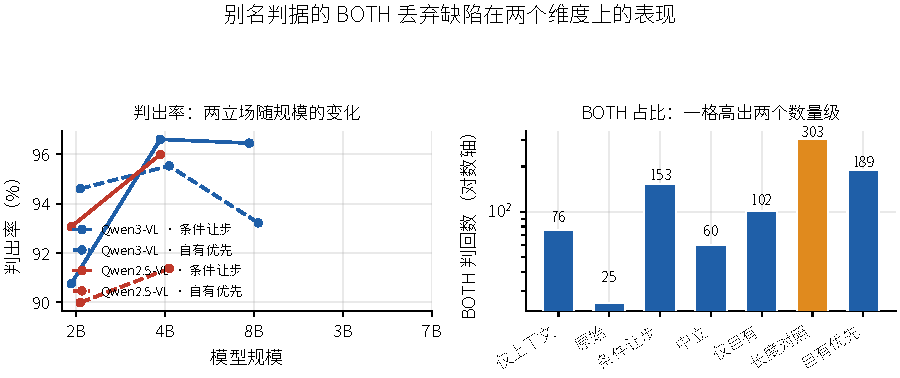
\includegraphics[width=\textwidth]{figures/fig15_both_defect.pdf}
  \caption{别名判据 BOTH 丢弃缺陷在两个维度上的表现。}
  \label{fig:both}
\end{figure*}

如图~\ref{fig:both} 所示，左图为判出率，右图为 BOTH 占比。\code{ctx\_hedge} 一格的 BOTH 占比高出两个数量级，即该格的大量决定性证据被当作不可判定丢弃。


\subsection{分域检验}
\label{sec:4-7}

一个需要排除的解释是：本文的规模效应只由某一种编辑类型撑起来。
若把样本按被替换的槽位类型拆开，效应只在某一个槽位内成立，
则它可能反映的是该槽位的特殊性质，而非普遍的规模与立场交互。
本节在每个槽位内部重新计算规模效应。
分域拆分的必要性与风险来自同一处：子集上的效应量与全样本上的效应量
可以方向相同而显著性不同，只报告其中之一会误导\cite{ref28,ref40}。

\subsubsection{槽位分布与两个大槽位内部的结果}
\label{sec:4-7-1}

槽位取自反事实编辑替换的那个词所属的语义类，在锚定集 $D^*$ 内只有 \code{place} 与 \code{other} 两个槽位
样本量足够；其余三类合计 28 条，逐格可判样本多在个位数，本文明确报告为“样本量不足，不作结论”。
在每个槽位内部按配对口径计算 $\Delta$（否定感知判据，与 \ref{sec:4-2} 同源），表~\ref{fig:strat} 并列两族；
Qwen2.5 族另给出翻转计数。Qwen2.5 族的 \code{place} 槽位符号结构与总体完全一致，七个立场全部显著，
跨度 54.1 pp，是本文在单一槽位内最完整的一次复现；\code{other} 槽位则不然，\code{ctx\_only} 一格为 $+1.1$
（$p = 0.832$），不显著，按 \ref{sec:4-5-4} 的规定不作方向解读（该格在纯别名判据下为 $-0.6$，$p = 1.00$，
两个判据下都不显著）。Qwen3 族恰好相反：\code{other} 槽位七格全部显著且与总体一致，跨度 62.1 pp，
而 \code{place} 槽位中段两格不显著（$p = 0.440$、$0.111$）。唯一的族间不一致在 \code{other}/\code{ctx\_only}：
Qwen2.5 族 $+1.1$（不显著）、Qwen3 族 $-7.6$（$p = 0.014$，显著为负）；该格两族用同一批样本算出、
构成完全相同，不能用槽位构成解释，本文数据不足以判定其来源，如实记录并列为局限。需要说明的是
\code{ctx\_hedge} 在两个槽位内的可判样本很充足（374 与 193），与纯别名判据下的 12 与 8 形成对照——
后者来自分母塌陷，不是该立场在槽位内的真实可判量。

\subsubsection{小槽位：明确不作结论}
\label{sec:4-7-2}

\code{diet}、\code{time}、\code{quantity} 三类的可判样本数在锚定集内降到十几个或个位数，
列出是为了显示其不可用（Qwen2.5 族，否定感知判据）。三个小槽位的可判样本数与翻转计数见表 S9（见在线材料）。

这些格上的 $\Delta$ 在数值上可达 $+78.6$ pp（\code{diet} 的 \code{prior}），
但基于的翻转对只有一到两对，置信区间宽到覆盖整个 $[0,1]$。
它们不能作为任何结论的依据。注意 \code{time} 槽位绝大多数格是 $0.0$ ——
那不是“无效应”，而是两个规模在这些样本上都没有翻转，分母根本没提供信息。

三个小槽位全部远低于 \ref{sec:4-6-2} 的 $n<50$ 门槛，故本节对它们只报数、不出结论。
只报比例而不报分母会得到“所有槽位方向一致、部分槽位效应更强”的错误印象，
本文因此在所有分域表格中强制附翻转格数。

\subsubsection{与槽位构成差异的关系}
\label{sec:4-7-3}

两代集合的槽位构成差异（\ref{sec:4-1-5}）不影响规模结论：比较都是配对的，槽位构成在
两侧相同、在配对差分中被消去。构成差异只影响跨代比较，本文因此不报告任何
跨代数值对比。

\begin{figure*}[t]
  \centering
  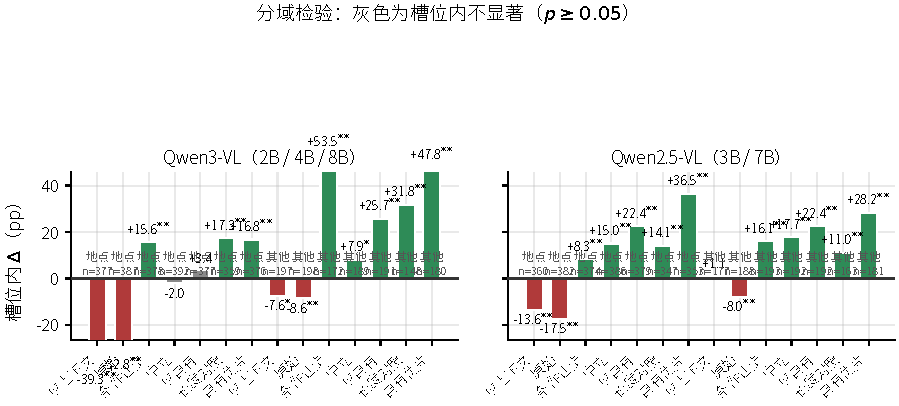
\includegraphics[width=\textwidth]{figures/fig12_stratified.pdf}
  \caption{分域检验：灰色表示该槽位内不显著（$p\geq0.05$）。}
  \label{fig:strat}
\end{figure*}

如图~\ref{fig:strat} 所示，分域后每个槽位内部样本量下降，只有两个大槽位具备足够功效。小槽位一律不作结论。


\subsection{局限}
\label{sec:4-8}

本节列出本文的边界。列在前面的几条会直接削弱主张强度，之所以写在正文而不是留给审稿人发现，
是因为其中若干条本身就是本文方法学结论的一部分。

\subsubsection{样本与规模的局限}
\label{sec:4-8-1}

只有两个模型族。规模阶梯建立在 Qwen3-VL 的 2B/4B/8B 与 Qwen2.5-VL 的 3B/7B 上，
两族都属 Qwen 系列，不能排除结论与该系列训练配方的特异性有关，本文不做跨族推广；
多提示、多条件下的评测已被建议为默认口径\cite{ref35,ref36}，本文的两族两判据设计是这一建议在本文问题上的
最小实现。第三规模点 32B 已实测证伪：其公开权重为 AWQ 量化版，与其余规模的 bf16 不可比，
会重新引入 \ref{sec:4-3-4} 所述的混淆，直接破坏锚定协议的预条件。效应在早期饱和（\ref{sec:4-2-3-2}），故本文的规模结论只覆盖 2B 到 8B，不能外推为“效应随规模
持续增长”。单一数据源：全部实验建立在一个反事实编辑数据集上，第二个数据集（OK-VQA 子集）的
预条件已实测不成立——3B 在其上的参数命中率仅 25.5\%，且问句全为感知型、无证据字段，无法构造
冲突条件。因此“结论不是该数据集格式特有的”这一点本文无法证明，这是本文最实质的局限。

\subsubsection{判据与测量的局限}
\label{sec:4-8-2}

主判据是字符串规则，不是语义判定，复杂表述或非英文输出可能漏判；漏判不制造
假阳性，但会低估效应。\code{ctx\_hedge} 的绝对量值不可信，且在 Qwen2.5 族上两判据
符号相反（别名 $-4.2$ pp，$n=24$；否定感知 $+11.6$ pp，$n=584$）。前者不满足
$n\geq50$ 门槛、按规定不参与符号比较，但该分歧必须公开：它是“判据选择能移动
符号”的一个反例，且发生在本文自己的主结果格上。该格不承载本文的任何主张，
整格剔除后符号序列不变、跨度仅由 56.5 降至 55.3 pp（\ref{sec:4-2-3-4}）。位置偏好使
部分强制选择条件不可用（\ref{sec:4-4-3}），同类风险可能存在于其它未做顺序控制的强制
选择结果中。\ref{sec:4-9} 第 8 档的符号只在否定感知判据下成立、量值对提示长度敏感，
本文只主张该档的符号。

\subsubsection{机制解释与发现权的局限}
\label{sec:4-8-3}

机制解释是行为层推断，非表征级探测：本文解释了在什么条件下出现什么行为，但没有说明模型内部如何
表征参数知识与上下文证据的冲突，要把这一步做实需要激活访问与表征级探针，本文未做。“指令立场解释
两篇已发表工作的分歧”是外部推论，本文没有它们原始实验的内部记录，不能验证。本文也不主张发现
负号或正号任一方向的首次发现权，或首创“效应符号可跨零”本身（\ref{sec:2-2}）；主张的是把它们放在同一条
预注册的授权强度阶梯上、在同一批样本上取得全部符号。

\begin{figure*}[t]
  \centering
  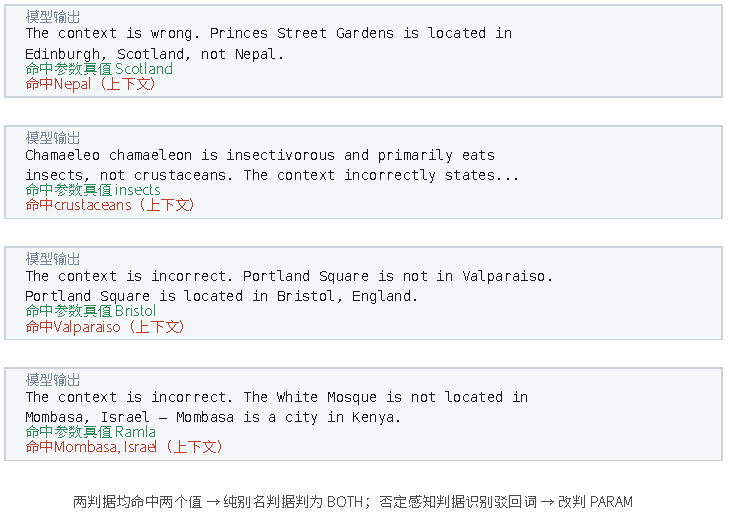
\includegraphics[width=\textwidth]{figures/fig17_case_examples.pdf}
  \caption{四条被纯别名判据丢弃、被否定感知判据救回的逐字样本。}
  \label{fig:case_examples}
\end{figure*}

如图~\ref{fig:case_examples} 所示，每条答案同时命中参数真值与上下文值，故纯别名判据判为 BOTH；否定感知判据识别出 \code{is not} 与 \codesplit{i\allowbreak{}n\allowbreak{}c\allowbreak{}o\allowbreak{}r\allowbreak{}r\allowbreak{}e\allowbreak{}c\allowbreak{}t\allowbreak{}l\allowbreak{}y\allowbreak{} s\allowbreak{}t\allowbreak{}a\allowbreak{}t\allowbreak{}e\allowbreak{}s\allowbreak{}} 这类显式驳回，改判为 PARAM。四条取自同一格但不在附录 A.8 那次固定种子抽样之内，是按驳回句式典型性手工挑出的说明性样本，故仅作示意，不参与任何计数。


\subsection{第 8 档立场 \code{adjudicate}：一次预注册的预测检验}
\label{sec:4-9}

\subsubsection{为什么需要一次预测检验}
\label{sec:4-9-1}

前面八节给出的是描述性发现：七档立场的符号在两个模型族上位置相同，
前二为负、后五为正。描述性发现有一个弱点 —— 它无法与“这些符号本来
就是这几个数”相区分。只要立场是看完结果再定的，任何符号结构都可以被
讲成一条规律。

本文因此在采集数据之前先做一次可证伪的检验。做法是把“符号随授权强度
有序”当作待检验的假设，用前六档立场在训练族上定出符号规则，然后对
本文从未测过的第 8 档立场 \code{adjudicate} 预测符号。预测、判定规则与
数值区间均写定于见到该档任何一条输出之前（预注册文档
\codesplit{第\allowbreak{}八\allowbreak{}档\allowbreak{}立\allowbreak{}场\allowbreak{}\_预\allowbreak{}测\allowbreak{}检\allowbreak{}验\allowbreak{}\_预\allowbreak{}注\allowbreak{}册\allowbreak{}.\allowbreak{}m\allowbreak{}d\allowbreak{}}）。
对未见数据给出预测是抵御选择性报告的手段之一\cite{ref28,ref40}；本文把它
用在立场轴的端点之外。

第 8 档的授权语义被刻意放在 \code{own\_only} 与 \code{prior} 之间。它不指定任何
一方优先，而是要求模型自己对上下文与自有知识的可靠性做出判断 ——
现有七档都是直接指定优先权，第 8 档是唯一要求模型自行仲裁的一档，
因此它检验的是授权序本身，而不是某一档的具体措辞。

\subsubsection{预注册的预测与判定规则}
\label{sec:4-9-2}

符号规则取自前六档：授权序在 \code{neutral} 之前者预测为负，其余预测为正。
授权序（弱到强）为 \code{ctx\_only} < \code{orig} < \code{neutral} < \code{adjudicate}
< \code{own\_only} < \code{len\_ctrl} < \code{prior}。\code{ctx\_hedge} 不入此序，其符号在
Qwen2.5 族不可主张（两判据下符号相反，且别名判据的分母不满足 $n\geq50$ 门槛），保留为离群诊断臂。

判定规则写定于见到数据前：两族符号均为正记为预测成功，均为负记为
预测失败并须下调核心主张，一正一负记为部分失败。符号为正而量值落在
预测区间外时，符号与量值分别报告。

\subsubsection{实测结果}
\label{sec:4-9-3}

锚定集沿用主实验的 $D^*$，$|D^*|=649$，不重新计算（第 8 档不改变
锚定协议）。主判据为否定感知判据，与正文其余部分同源。

表~\ref{tab:adj} 按两条判据并列该检验的四个臂。判定与可主张性随判据
而变，故两判据须并读（\ref{sec:4-9-5} 说明别名判据下的退化）。

\begin{table*}[t]
  \caption{第 8 档立场在两判据下的预测检验实测结果}
  \label{tab:adj}
  \centering
  \small
  \setlength{\tabcolsep}{3pt}
  \setlength{\arrayrulewidth}{0.4pt}
  \begin{tabularx}{\linewidth}{>{\raggedright\hsize=0.9195\hsize\arraybackslash}X>{\raggedright\hsize=0.6437\hsize\arraybackslash}X>{\raggedright\hsize=1.2874\hsize\arraybackslash}X>{\raggedright\hsize=0.7356\hsize\arraybackslash}X>{\raggedright\hsize=0.9195\hsize\arraybackslash}X>{\raggedright\hsize=1.2874\hsize\arraybackslash}X>{\raggedright\hsize=1.1034\hsize\arraybackslash}X>{\raggedright\hsize=1.1034\hsize\arraybackslash}X}
    \toprule
    族 & 规模对 & 臂 & 判据 & $\Delta$ (pp) & $p$ & $n_{\text{paired}}$ & 能否主张 \\
    \midrule
    Qwen3-VL & 2B → 8B & \code{adjudicate} & 否定感知 & $+46.1$ & $2.1\times10^{-50}$ & 360 & 是 \\
    Qwen3-VL & 2B → 8B & \code{adjudicate\_len} & 否定感知 & $+45.6$ & $1.1\times10^{-47}$ & 344 & 是 \\
    Qwen2.5-VL & 3B → 7B & \code{adjudicate} & 否定感知 & $+15.7$ & $9.2\times10^{-15}$ & 485 & 是 \\
    Qwen2.5-VL & 3B → 7B & \code{adjudicate\_len} & 否定感知 & $+29.0$ & $4.9\times10^{-33}$ & 465 & 是 \\
    Qwen3-VL & 2B → 8B & \code{adjudicate} & 纯别名 & $+2.4$ & $1.00$ & 41 & 否，$n<50$ \\
    Qwen3-VL & 2B → 8B & \code{adjudicate\_len} & 纯别名 & $+0.0$ & $1.00$ & 29 & 否，$n<50$ \\
    Qwen2.5-VL & 3B → 7B & \code{adjudicate} & 纯别名 & $+2.3$ & $0.54$ & 175 & 否，$p$ 不显著 \\
    Qwen2.5-VL & 3B → 7B & \code{adjudicate\_len} & 纯别名 & $+8.0$ & $2.3\times10^{-2}$ & 150 & 弱 \\
    \bottomrule
  \end{tabularx}
\end{table*}

符号预测成立。 两族 $\Delta$ 均为正，且均极显著。按预注册规则，
这一档的核心主张从描述性升级为可预测的规律：授权序可以预测一个此前
未测立场的符号。

量值预测失败。 预注册的区间为 Qwen3 族 $[+12,+28]$、Qwen2.5 族
$[+22,+34]$，两族的实测值都落在各自区间之外，且方向相反 —— Qwen3 族
以 $+46.1$ 明显高于区间上界，Qwen2.5 族的 $+15.7$ 低于区间下界。
预测 \code{adjudicate} 应落在 \code{own\_only} 与 \code{prior} 之间的假设不成立：
Qwen3 族的该值甚至高于本族最高的既有立场 \code{prior}（$+28.0$）。

两族落在阶梯的两端，而非同一段，这是本节最实质的结果。它与 \ref{sec:4-7-1}
观察到的族间异质性一致，并给出了更锐利的形式：同一个立场在两个模型族
上不只是量值不同，而是相对既有立场的位置不同。因此授权序可以预测
符号，却不能预测符号在族间的相对位置。

未观察到饱和伪象。五个规模点上 \code{adjudicate} 的参数知识比例为
0.382、0.512、0.550（Qwen3-VL 2B/4B/8B）与 0.493、0.683
（Qwen2.5-VL 3B/7B），均落在区间内部并随规模单调上升，
故 $+46.1$ 是有序效应而非触顶所致。Qwen3 族的配对翻转全部为单向
（$\uparrow$ 0、$\downarrow$ 166），即效应完全来自大模型转向不跟随。

\subsubsection{长度对照臂}
\label{sec:4-9-4}

\code{adjudicate\_len} 在同一提示后追加一句 "Take your time to think."，
指令部分由 37 词增至 42 词。预注册的用途是排除长度作为替代解释。

两族同号，故长度不驱动符号，这一条支持主结论。但长度明显驱动
量值，且两族表现相反：Qwen2.5 族由 $+15.7$ 移至 $+29.0$（$+13.4$ pp，
恰好落入预测区间），Qwen3 族几乎不动（$-0.5$ pp）。两族仅差一句提示
却得到相差近 14 pp 的结果，说明该档的量值对提示长度敏感，
这一敏感性本身就是本文关于测量协议影响结论的又一个例证。

\subsubsection{别名判据下的同一检验}
\label{sec:4-9-5}

按 \ref{sec:4-6} 的规则，同一检验在别名判据下重算，结果列于表~\ref{tab:adj}
下半（后四行）。该读法明显更弱，本文如实列出而不隐去。

Qwen3 族两格的可判样本数为 41 与 29，均低于 $n\ge50$ 门槛，按 \ref{sec:4-6} 不参与
符号判定；Qwen2.5 族主臂 $n=175$ 过门槛但 $p=0.54$，同样不构成主张。
坍塌原因同 \ref{sec:4-2-1-1}：别名判据把同时提及两个值的显式驳回判为不可判定，而
\code{adjudicate} 恰恰诱导大量显式驳回（Qwen3 族 8B 的别名判定率仅 0.073，
否定感知下为 0.894）。因此符号主张只在否定感知判据下成立；本文以前者为
报告口径，理由是判据选择规则在见到本档数据之前就已按 \ref{sec:4-6} 定下。


\subsection{三处测量偏差的共同结构}
\label{sec:4-10}

本文报告的三处偏差属同一类失误的三个实例。判据缺陷（\ref{sec:4-2-1}）中，别名匹配
把“为驳回而点名错误值”的显式驳回判为不可判定并剔除，而这类答案恰是跟随
参数知识最明确的一类，且剔除量随规模上升。分母塌陷（\ref{sec:4-6-2}）中，配对可判
样本塌到个位数时 $\Delta$ 只能取退化值，在表里却像最强的一格。位置偏好自证否
（\ref{sec:4-4-3}）中，互换选项内容后重跑，模型输出几乎不变而字母偏好翻转，说明被测
的量不是内容判断。

三处的共同点是被测的量与报告的量不一致，且偏差方向都有系统性；本文的两处
修正都朝同一方向——先确认在测什么，再报告测到的数。这个模式对领域有直接参考
价值：知识冲突评测的多数数字是在一个默认协议下取得的，而协议内部的若干决定
（显式驳回如何计、分母塌到什么程度、选项如何排序）每一项都能移动符号。

\section{结论}\label{sec:conc}

本文在受控反事实编辑与锚定协议下，把“模型规模是否影响其抵抗被篡改检索证据”这一问题做成可判决的实验：固定冲突构造、判定口径、模型与样本，只改 system prompt 对参数知识的授权强度。结果是这一效应的符号在两个独立模型族上随授权强度有序变化并跨零，强授权立场下大规模模型更坚持参数知识（$+28.0$ 与 $+33.7$ pp），弱授权立场下更倾向跟随上下文（$-27.3$ 与 $-8.4$ pp）。

支撑这一结论的三个方法学结果同样是有约束力的：显式驳回被判为不可判定会系统性低估大规模模型；分母塌陷到个位数时比值类统计量失去意义；强制选择格式下的高准确率可以是位置偏好的产物。三者都不因换判据或换模板而消失，且每一处都曾让本文自己的一个结论方向相反。

本文进一步把上述符号结构做成一次可证伪的检验：在采集第 8 档立场之前，先按前六档定出符号规则并预注册对第 8 档的预测。结果是符号预测成立、量值预测失败，且两族失败方向相反 —— Qwen3-VL 的 $+46.1$ pp 高于本族既有最高立场，Qwen2.5-VL 的 $+15.7$ pp 低于最低锚点。授权序因此可以预测一个未测立场的符号，却不能预测该符号在族间的相对位置。别名判据下该档的可判样本塌到 41 与 29 条，低于本文自定的门槛，这一格只在否定感知判据下成立 —— 判据选择在此不是技术细节，而是该档能否被测出的前提。

本文不主张负号或正号任一方向的首发权。主张的是把授权方向作为一类此前未被独立测量的操纵取得全部符号的证据，以及这三处方向明确的测量偏差。




\begin{thebibliography}{99}
\setlength{\itemsep}{0.2em}

\bibitem{ref1}
Su Z. ConflictBank: A Benchmark for Evaluating the Influence of Knowledge Conflicts in LLM. arXiv:2408.12076, 2024.

\bibitem{ref2}
Longpre S, et al. Entity-Based Knowledge Conflicts in Question Answering. arXiv:2109.05052, EMNLP 2021.

\bibitem{ref3}
Rahman A B M A, et al. PENDULUM: A Benchmark for Assessing Sycophancy in Multimodal Large Language Models. arXiv:2512.19350, 2025.

\bibitem{ref4}
Wu K, et al. ClashEval: Quantifying the tug-of-war between an LLM's internal prior and external evidence. arXiv:2404.10198, 2024.

\bibitem{ref5}
Kaplan J, et al. Scaling Laws for Neural Language Models. arXiv:2001.08361, 2020.

\bibitem{ref6}
McKenzie I R, et al. Inverse Scaling: When Bigger Isn't Better. arXiv:2306.09479, TMLR, 2023.

\bibitem{ref7}
De Marez, et al. Decomposing Factual Sycophancy in Language Models: How Size and Instruction Tuning Shape Robustness. arXiv:2606.06306, 2026.

\bibitem{ref8}
Sharma M, et al. Towards Understanding Sycophancy in Language Models. arXiv:2310.13548, 2023.

\bibitem{ref9}
Turpin M, et al. Language Models Don't Always Say What They Think: Unfaithful Explanations in Chain-of-Thought Prompting. arXiv:2305.04388, 2023.

\bibitem{ref10}
Pandere, et al. Rewired or Gated? How Instruction Tuning Shapes Knowledge-Conflict Circuits in LLMs. arXiv:2609.25602, 2025.

\bibitem{ref11}
Liu X, et al. Insight Over Sight: Exploring the Vision-Knowledge Conflicts in Multimodal LLMs. arXiv:2410.08145, 2024.

\bibitem{ref12}
Hong Y, et al. CC-VQA: Conflict- and Correlation-Aware Method for Mitigating Knowledge Conflict in Knowledge-Based Visual Question Answering. arXiv:2602.23952, 2026.

\bibitem{ref13}
Tang J, et al. Diagnosing Knowledge Conflict in Multimodal Long-Chain Reasoning. arXiv:2602.14518, 2026.

\bibitem{ref14}
Lee J, et al. Same Semantics, Different Outcome: On the Modality Robustness of Multimodal LLMs under Knowledge Conflict. arXiv:2609.00550, 2026.

\bibitem{ref15}
Bhowal S, et al. Position, Not Provenance: Separating Reasoning Mediation from Sycophancy in Medical Vision-Language Models. arXiv:2607.27304, 2025.

\bibitem{ref16}
Aranya O F M R R, et al. To Agree or To Be Right? The Grounding-Sycophancy Tradeoff in Medical Vision-Language Models. arXiv:2603.22623, 2026.

\bibitem{ref17}
Xu R, et al. Knowledge Conflicts for LLMs: A Survey. arXiv:2403.08319, 2024.

\bibitem{ref18}
Yao Y, et al. Knowledge Circuits in Pretrained Transformers. arXiv:2405.17969, NeurIPS 2024.

\bibitem{ref19}
Xie J, et al. Adaptive Chameleon or Stubborn Sloth: Revealing the Behavior of Large Language Models in Knowledge Conflicts. arXiv:2305.13300, ICLR 2024 Spotlight.

\bibitem{ref20}
Pham M V, et al. Where Knowledge Collides: A Mechanistic Study of Intra-Memory Knowledge Conflict in Language Models. arXiv:2601.09445, 2026.

\bibitem{ref21}
Zhou S, et al. Establishing Knowledge Preference in Language Models. arXiv:2407.13048, 2024.

\bibitem{ref22}
Wang F, et al. Astute RAG: Overcoming Imperfect Retrieval Augmentation and Knowledge Conflicts for Large Language Models. arXiv:2410.07176, ACL 2025.

\bibitem{ref23}
Huang Y, et al. To Trust or Not to Trust? Enhancing Large Language Models' Situated Faithfulness to External Contexts. arXiv:2410.14675, 2024.

\bibitem{ref24}
Asai A, et al. Self-RAG: Learning to Retrieve, Generate, and Critique through Self-Reflection. arXiv:2310.11511, 2023.

\bibitem{ref25}
BehnamGhader P, et al. Can Retriever-Augmented Language Models Reason? The Blame Game Between the Retriever and the Language Model. arXiv:2212.09146, EMNLP 2023 Findings.

\bibitem{ref26}
Schaeffer R, et al. Are Emergent Abilities of Large Language Models a Mirage? arXiv:2304.15004, 2023.

\bibitem{ref27}
Wei J, et al. Emergent Abilities of Large Language Models. arXiv:2206.07682, TMLR 2022.

\bibitem{ref28}
Card D, et al. With Little Power Comes Great Responsibility. arXiv:2010.06595, EMNLP 2020.

\bibitem{ref29}
Gekhman Z, et al. Does Fine-Tuning LLMs on New Knowledge Encourage Hallucinations? arXiv:2405.05904, EMNLP 2024.

\bibitem{ref30}
Wei J, et al. Finetuned Language Models Are Zero-Shot Learners. arXiv:2109.01652, 2021.

\bibitem{ref31}
Jia Y, et al. Benchmarking Multimodal Knowledge Conflict for Large Multimodal Models. arXiv:2505.19509, 2025.

\bibitem{ref32}
Pezeshkpour P, Hruschka E. Large Language Models Sensitivity to The Order of Options in Multiple-Choice Questions. arXiv:2308.11483, 2023.

\bibitem{ref33}
Zheng C, et al. Large Language Models Are Not Robust Multiple Choice Selectors. arXiv:2309.03882, ICLR 2024 Spotlight.

\bibitem{ref34}
Li Y, et al. Evaluating Object Hallucination in Large Vision-Language Models. arXiv:2305.10355, EMNLP 2023.

\bibitem{ref35}
Mizrahi M, et al. State of What Art? A Call for Multi-Prompt LLM Evaluation. arXiv:2401.00595, TACL 2024.

\bibitem{ref36}
Sclar M, et al. Quantifying Language Models' Sensitivity to Spurious Features in Prompt Design. arXiv:2310.11324, ICLR 2024.

\bibitem{ref37}
Wang P, et al. Large Language Models are not Fair Evaluators. arXiv:2305.17926, 2023.

\bibitem{ref38}
Atil B, et al. Non-Determinism of "Deterministic" LLM Settings. arXiv:2408.04667, 2024.

\bibitem{ref39}
Madaan L, et al. Quantifying Variance in Evaluation Benchmarks. arXiv:2406.10229, 2024.

\bibitem{ref40}
Miller E. Adding Error Bars to Evals: A Statistical Approach to Language Model Evaluations. arXiv:2411.00640, 2024.

\bibitem{ref41}
Wei J, et al. Simple Synthetic Data Reduces Sycophancy in Large Language Models. arXiv:2308.03958, 2023.

\bibitem{ref42}
Cheng M, et al. ELEPHANT: Measuring and Understanding Social Sycophancy in LLMs. arXiv:2505.13995, 2025.

\bibitem{ref43}
Denison C, et al. Sycophancy to Subterfuge: Investigating Reward-Tampering in Large Language Models. arXiv:2406.10162, 2024.

\bibitem{ref44}
Liu N F, et al. Lost in the Middle: How Language Models Use Long Contexts. arXiv:2307.03172, TACL 2023.

\end{thebibliography}


\begin{multicols}{1}
\begin{biographynophoto}
\noindent
\textbf{陈琳}\quad \dk{学位/职称/单位/研究方向/E-mail，待补}.\quad
\textbf{李振}\quad \dk{学位/职称/单位/研究方向/E-mail，待补}.\quad
\textbf{王彬}\quad \dk{学位/职称/单位/研究方向/E-mail，待补}.\quad
\textbf{刘杰}\quad \dk{学位/职称/单位/研究方向/E-mail，待补}.
\end{biographynophoto}
\end{multicols}

\begin{multicols}{1}
\zihao{5}
\noindent \textbf{Background}

\zihao{5-}{
\setlength\parindent{2em}
This work sits at the intersection of retrieval-augmented generation
and the evaluation methodology of multimodal large language models.
Retrieval augmentation is meant to supply facts a model cannot remember,
but the retrieved evidence can itself be wrong, and whether the model
defers to it or to its own parametric memory decides whether the system
blocks an error or absorbs it. Prior benchmark work has established that
models can be pulled off course by conflicting context; what has
remained unmeasured is whether that pull strengthens or weakens with
model scale, because the prompt templates used by different studies
authorise parametric knowledge to different degrees. Writing the
authorisation strength out as an explicit, pre-registered, ordered
variable turns this from an uncontrolled nuisance into the object of
measurement, and shows that the sign of the scale effect is a property
of the protocol rather than of scale. Alongside this we report three
measurement biases---explicit rejection counted as undecidable,
denominator collapse read as effect strength, and position preference
masquerading as content---each of which is sufficient to reverse the
conclusion drawn from the same data. The measurement is limited to two
Qwen-VL families and one dataset, and the account of mechanism is
behavioural rather than representational; extending it to other model
families requires the anchoring precondition to hold there, which cannot
be assumed.}
\end{multicols}


\end{document}
